%-----------------------------------------------------------------------------
%
%               Template for LaTeX Class/Style File
%
% Name:         sigplanconf-template.tex
% Purpose:      A template for sigplanconf.cls, which is a LaTeX 2e class
%               file for SIGPLAN conference proceedings.
%
% Author:       Paul C. Anagnostopoulos
%               Windfall Software
%               978 371-2316
%               paul@windfall.com
%
% Created:      15 February 2005
%
%-----------------------------------------------------------------------------


%\documentclass[preprint]{sigplanconf}
\documentclass{sigplanconf}

\usepackage{amsmath}
%\usepackage[frenchb,english]{babel}
\usepackage{graphicx}

\begin{document}

\conferenceinfo{PEPM'08,}{January 7--8, 2008, San Francisco, California, USA.}
\CopyrightYear{2008}
\copyrightdata{978-1-59593-977-7/08/0001} 

%\titlebanner{banner above paper title}        % These are ignored unless
%\preprintfooter{short description of paper}   % 'preprint' option specified.

\title{Unparsed Patterns: Easy User-Extensibility of Program
Manipulation Tools\thanks{This extended version contains an extra
Appendix with the proof of the claimed properties. This Appendix has
been omitted in the published PEPM'08 version because of space
limitations.}}

\subtitle{Extended Version}

\authorinfo{Nic Volanschi}
           {{\em my}{\bf gcc}}
           {nic.volanschi@free.fr}
\authorinfo{Christian Rinderknecht}
           {Konkuk University \\ 
	     143-701 Seoul Gwangjin-gu Hwayang-dong \\
	     South Korea}
           {rinderkn@konkuk.ac.kr}

\maketitle

\begin{abstract}
Pattern matching in concrete syntax is very useful in program
manipulation tools. In particular, user-defined extensions to such
tools are written much easier using concrete syntax patterns. A few
advanced frameworks for language development implement support for
concrete syntax patterns, but mainstream frameworks used today still
do not support them. This prevents most existing program manipulation
tools from using concrete syntax matching, which in particular
severely limits the writing of tool extensions to a few language
experts.

This paper argues that the major implementation obstacle to the
pervasive use of concrete syntax patterns is the pattern parser. We
propose an alternative approach based on ``unparsed patterns'', which
are concrete syntax patterns that can be efficiently matched without
being parsed. This lighter approach gives up static checks that parsed
patterns usually do. In turn, it can be integrated within any existing
parser-based software tool, almost for free. One possible consequence
is enabling a widespread adoption of extensible program manipulation
tools by the majority of programmers.

Unparsed patterns can be used in any programing language, including
multi-lingual environments. To demonstrate our approach, we
implemented it both as a minimal patch for the gcc compiler, allowing
to scan source code for user-defined patterns, and as a standalone
prototype called matchbox.
\end{abstract}

\category{D.3.3}{Language Constructs and Features}{Patterns}

\terms Algorithms, Languages

\keywords
pattern matching, source code, unparsed patterns

%%-*-latex-*-

\section{Introduction}
Pattern matching of source code is a very useful mechanism in tools
for program analysis and transformation, such as compilers,
interpreters, tools for legacy program understanding, code inspectors,
refactoring tools, model checkers, code translators, etc. Source code
matching is not only useful when implementing these tools, but
especially for building extensible versions of these tools with
user-defined behavior \cite{mc, mj, mops, blast, mygcc, pmd}.

As the problem of tree matching has been
extensively studied and efficient algorithms are known, the problem of
source code matching has usually been reduced to tree matching,
according to two different approaches.

\paragraph{Tree patterns.}
In the first approach, code patterns are written as trees, using a
domain-specific notation to describe an abstract syntax tree
(AST). This approach based on tree patterns has been used for a long
time, either supported by pattern matching mechanisms available in the
implementation language, e.g., for tools written in ML, or otherwise
by explicitly implementing a tree pattern matching mechanism, e.g. in
inspection tools such as tawk \cite{tawk} or SCRUPLE \cite{scruple} or
in model checking tools such as MOPS \cite{mops}. More recently, some
extensible code inspectors such as PMD \cite{pmd} represent ASTs in
XML notation (which constitutes a standardized notation for
trees). This allows using other standardized notations such as
XPath/XQuery for expressing tree patterns, and thus reusing existing
pattern matchers. The main advantage of expressing patterns as trees
is that the implementation of pattern matching is simple, because any
appropriate tree-matching algorithm can be directly used on this
representation. However, an important shortcoming of this approach is
that programmers writing patterns should be aware of the internal AST
representation of programs, and also of a specific notation for it.

As a motivating example, consider a very simple user-defined
inspection rule over C programs that searches for code fragments
resetting all the elements in an array, such as the following
fragment:
\begin{verbatim}
for(i=0; i<100; ++i)
  a[i]=0;
\end{verbatim}
When such initialization code is found, the inspection rule may
suggest that the same operation would be implemented more efficiently
using the ``bzero()'' standard library function. Alternatively, the
same rule might be predefined in a compiler in order to recognize such
initializations and automatically implement them more efficiently
using the ``bzero()'' function.

Depending on the AST representation of the C program in a particular
tool, the tree pattern corresponding to the example above would
typically be expressed as follows (where the name of the array, its
bound, and its index variable have been abstracted as variables in the
pattern):
\begin{verbatim}
for_stmt(assign_expr(X, N), 
         less_expr(X, M), 
         preincr_expr(X),
         expr_stmt(assign_expr(array_expr(Y, X), 
                               int_literal(0))))
\end{verbatim}

As can be seen in the above tree pattern, the programmer writing the
inspection rule must be aware of both the AST structure (for instance,
that an assignment in C is an expression encapsulated in an
``expression statement'') and of a specific notation for it (for
instance, that the assignment operator is called ``assign\_expr'',
that the ``for\_stmt'' operator takes four arguments in a given order,
etc.). Writing the same pattern in a language such as XPath doesn't
simplify things, and the pattern becomes even more verbose.

\paragraph{Concrete syntax patterns.}
In the second approach to source code matching, code patterns are
expressed using the native syntax (i.e., the concrete syntax) of the
subject programming language, augmented with pattern variables. Then,
patterns are parsed to trees before being matched with the program
AST. In this approach, the pattern to be searched can be written much
more naturally and concisely as follows (where variables in the
pattern are prefixed by a special character such as ``\%''):
\begin{verbatim}
for(%x=0; %x<%n; ++%x) %y[%x]=0;
\end{verbatim}

This second approach based on concrete syntax patterns has been used,
for instance, in several extensible model checkers \cite{cecil, mc,
mj, blast}, and extensible tools for legacy program understanding and
transformation \cite{native, behavioral}. The main advantage of
concrete syntax patterns is that they are trivial to write and read
back by any programmer, without knowledge of the AST
representation. However, as far as the implementation is concerned,
parsing the pattern requires a modified parser of the subject
programing language, extended to:
\begin{itemize}
\item allow pattern variables, which do not occur in ordinary code, and
\item parse patterns that represent program {\em fragments}
(statements, expressions, declarations), whereas the base grammar only
parsed whole programs.
\end{itemize}
Extending the parser of a programing language in these ways is not a
simple task, even in frameworks that automate the addition of the
extra grammar productions \cite{refine}, because it typically
introduces many conflicts in the parser. These conflicts may
correspond to real ambiguities in the extended language (for example,
in C, the pattern ``f(\%x);'' may represent either a function call or
a function declaration with an implicit return type of ``int''), or
may be just be caused by a parsing algorithm with limited
lookahead. Indeed, existing parsers most commonly use limited
lookahead algorithms such as LALR(1) or LL(1). Solving many such
conflicts in a complex grammar of a real programming language may be
very hard to do. Moreover, the resolution of some conflicts may
require introducing special pattern syntax (such as ``\#stmt f(\%x);''
in the previous example), which make the patterns look less similar to
native code. This is the reason why most of the existing tools
following this approach allow only restricted forms of concrete syntax
patterns, described by a limited pattern grammar (e.g., matching only
assignments and function calls \cite{blast-ql}).

In theory, generalized parsers, handling the general class of
context-free grammars, can deal with both kinds of conflicts, by
computing all possible parses: conflicts due to limited lookahead are
rejected later during the parsing; conflicts due to the ambiguity of
the grammar itself result in several possible ASTs. However,
mainstream generalized parsers such as Bison \cite{bison} use an
extremely inefficient, exponential-time algorithm, creating a new
process at each local ambiguity. This scheme may quickly prove
infeasible when parsing even small fragments in a pattern grammar
where conflicts are scattered everywhere.

Alternatively, the polynomial-time GLR parsing algorithm \cite{glr}
was used to implement tools such as SDF \cite{sdf}, used by ASF+SDF
\cite{asf+sdf} and Stratego/XT \cite{metaprog} to implement concrete
syntax rewriting rules, or very recently BRNGLR \cite{brnglr}. Even
so, there is still a performance issue, because GLR parsers are
typically much less efficient than LALR(1) parsers (a factor of 10 is
not uncommon \cite{elkhound}). Also recently, a hybrid GLR/LALR parser
called Elkhound \cite{elkhound} has been delivered whose running time
is close to that of a standard LALR(1) parser on all the portions of a
grammar that are LALR(1). But as discussed above, an extended pattern
grammar is highly ambiguous (unless we severely restrict the
patterns), so then GLR parsing time would fall back to usual GLR-class
performance. Therefore, GLR parsing may not be in general an
efficient, production-quality, solution to the problem of parsing
source code patterns. Other generalized parsing algorithms such as
Earley \cite{earley} may eventually perform better on such highly
ambiguous grammars.

Besides this performance issue, there is also an even more important
porting issue, when talking about legacy parsers. Indeed, for either
performance or historical reasons, generalized parsers are very rarely
used in existing tools. Porting an existing parser to a different
technology may be difficult --- typically, the grammar has to be
rewritten from scratch. Furthermore, rewriting the parser may
profoundly impact the rest of the tool. This effort is simply
unaffordable for most legacy tools.

\paragraph{Our solution.}
Summarizing, there is no simple solution today for adding concrete
syntax pattern matching in existing parser-based tools without either
profoundly restructuring the parser, rewriting it in another
framework, severely restricting the patterns, or compromising
performance. As a consequence, concrete patterns are rarely used in
existing parser-based tools such as mainstream compilers. In
particular, the lack of concrete patterns is particularly limiting
the implementation of convenient user extensions in tools such as
extensible compilers, code inspectors, model checkers, etc.

To solve this problem in a pragmatic way, we designed a pattern
matching technique based on ``unparsed patterns'', that allows using
efficient, unrestricted, concrete syntax patterns while requiring no
extension of the parser for the subject programing language. In
particular, this technique is applicable to existing parsers, based on
any parsing technology, without porting them to a different framework.

In a previous paper \cite{ppdp}, we showed some concrete application
of unparsed patterns within a checking compiler called mygcc. That
application paper first introduced the idea of unparsed patterns, and
briefly mentioned that they work by unparsing the AST, rather than
parsing the pattern. However, no details were previously published
about their implementation, nor about the theoretical aspects raised
by these patterns. Both are the subject of the current paper. As we
will show in the following, the simple idea of unparsing the AST must
be combined non-trivially with other ingredients in order to obtain
a usable pattern matching algorithm.

The main contributions of this paper can be summarized as follows:
\begin{itemize}
\item we describe in detail the novel paradigm of pattern matching of
source code in concrete syntax, based on unparsing;
\item we describe a family of linear-time pattern matching algorithms
combining in different ways: unparsing, laziness, token analysis,
lookahead and parenthesizing;
\item we show how our pattern matching technology can be implemented
in a completely language-independent way;
\item from a theoretical point of view, our approach goes beyond the
presented algorithms, by opening a series of interesting questions
about: optimal parenthesizing, classes of grammars needing no
parentheses in the patterns, pattern extensions, etc.;
\item from a practical point of view, we expect that our approach will
have a significant impact on existing parser-based tools written in
imperative languages, by providing them pattern matching at a minimal
cost, as demonstrated by our very concise implementation within the
gcc compiler.
\end{itemize}

The rest of this paper is organized as follows. Section~\ref{defs}
defines unparsed patterns. Section~\ref{informal} informally describes
and Section~\ref{algos} precisely defines a family of pattern matching
algorithms for unparsed patterns. Section~\ref{implem} describes two
implementations of unparsed patterns. Section~\ref{assess} puts into
perspective unparsed patterns. Section~\ref{relwork} discusses related
work and Section~\ref{concl} concludes.


\section{Unparsed patterns}
\label{defs}
{\em Unparsed patterns} are a particular form of concrete syntax
patterns: they are written using the native syntax of the underlying
programming language, except that they may contain pattern
variables. Pattern variables may replace any sub-construct of a
program fragment that is represented by a subtree in the AST. For
example, pattern variables may replace any subexpression of an
expression or of a statement; the ``then'' or ``else'' branch of a
conditional, etc. Pattern variables are sometimes called
meta-variables, to distinguish them from the variables of the subject
programming language.

We illustrate the notion of unparsed patterns mainly in the context of
C programs, but the idea is completely language-independent, and we
occasionally give examples in other languages.

Unparsed patterns are always represented as quoted strings, in which
pattern variables are preceded by an escape character. The escape
character used in this paper is ``\%'', adhering to the familiar
convention used for C ``format strings'', but any other escape
sequence can be used. For example, ``buf = malloc(sizeof(int));'',
``\%x = malloc(\%y);'', ``\%l = \%l-\verb.>.next;'' are unparsed
patterns representing C statements, and ``\%x = malloc(\%y)'' (without
the ending semicolon), ``\%x \verb.>.= threshold'', and ``p == NULL''
are unparsed patterns representing C (or C++, or Java) expressions.

A {\em program fragment} is a substring of contiguous program source
text that can be parsed entirely as a single AST. For example, ``x +
(y/2)'', ``y=0; x=1;'', and ``while(i-\,-) /* update p */ *p++;'' are
program fragments, while ``if(p!=0)'', ``x='', and `` (sizeof(int''
are not program fragments. The AST of a program fragment ``f'' is
noted AST(``f''). Note that several program fragments, differing only
in whitespace, comments, and redundant parentheses, may correspond to
the same AST.

The {\em unparsed string} of an AST $t$, noted TXT($t$), is the string
obtained by ``unparsing'' $t$, i.e. by recursively printing the
concrete syntax of $t$ in a standard way, with no comments and with
sufficient whitespace and parentheses to make the text parsable back
to $t$. Ideally, the unparsed string should not contain redundant
whitespace and parentheses. The unparsed string of an AST $t$
obviously is a program fragment, its AST being $t$ itself.

An AST $t$ is said to {\em match} an unparsed pattern $p$ containing
meta-variables $x_i$ if there is a substitution $\{x_i\gets t_i\}$
where $t_i$ are subtrees of $t$ such that $TXT(t) = p[x_i\gets
TXT(t_i)]$.  If we use the corresponding textual substitution
$\sigma^{TXT}=\{x_i\gets TXT(t_i)\}$, we can write the above condition
in a simpler way: $TXT(t) = \sigma^{TXT}(p)$

In the previous equality, the first term represents the unparsed
string of the AST, and the second term represents the instantiated
unparsed pattern, obtained by substituting in the pattern all
variables by the unparsed string of their bound subtree.

By extension, a program fragment is said to match an unparsed pattern
if its AST matches the pattern. We also say sometimes that
the pattern matches the program fragment.

The above definition of pattern matching implies that a same variable
occurring several times in a pattern must stand for the same subtree
(in other words, non-linear patterns are correctly handled). However,
for cases where the value of the variable is not important, there is
an anonymous variable, noted ``\%\_'' in the patterns, that is always
free. The anonymous variable is a special case in that different
occurrences of it in the same pattern may be bound to different
subtrees.

For instance, the pattern ``\%l = \%l-\verb.>.next;'' matches the
statement ``list = list-\verb.>.next;'' under the substitution
$\{l\gets AST(\mbox{``list''})\}$. We sometimes write the resulting
substitution simply $\{l\gets list\}$, where the subtrees are denoted
by their unparsed strings. The same pattern does not match the
statement ``p = buf[0]-\verb.>.next;''.

%% Note that there are not two distinct types of patterns, one for
%% statements and another for expressions: it just happens that some
%% patterns may match only statements, while some other may match only
%% expressions. For example, all the patterns ending in ``;'' will match
%% only C statements, never C expressions.

\section{Matching unparsed patterns}
\label{informal}
Before presenting precise algorithms for unparsed pattern matching in
Section~\ref{algos}, we discuss them informally on a running
example. Consider the problem of matching the C expression ``a = a - b
* c - d'' with the code pattern ``\%x = \%y - \%z''.

%% \subsection{Comparison to existing approaches}
%% Plain string matching is very imprecise, because it would allow to
%% bind both $\{x\gets a, y\gets a-b*c, z\gets d\}$, which is correct, and
%% $\{x\gets a, y\gets a, z\gets b*c-d\}$, which is incorrect, since the
%% subtraction operator is left-associative. It even would match the
%% expression with the pattern ``\%x = \%y * \%z'', which is a complete
%% non-sense in terms of C. This is clearly because the structure
%% information contained in the AST is absent in the equivalent string.

%% Of course, more precise code pattern matching can be achieved by
%% performing it on the AST representation of a program. Traditional
%% approaches reduce the problem to pattern matching between two trees,
%% either by providing the pattern directly in a tree form or by parsing
%% it down to a tree form.

Traditional, parser-based, pattern matching would first parse the
expression using the usual program parser down to the AST in
Figure~\ref{fig:treematch}(a), parse the pattern using an extended
pattern parser to the tree in Figure~\ref{fig:treematch}(b), and then
match the two trees, finally binding pattern variables in the only
correct way: $\{x\gets a, y\gets a-b*c, z\gets d\}$.
\begin{figure}
\centering
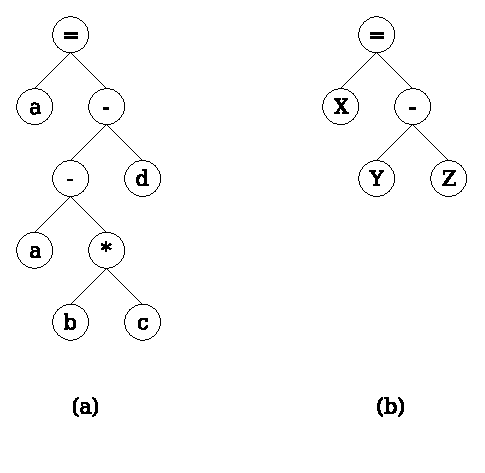
\includegraphics[width=6cm]{treematch.eps}
\caption{Matching AST(``a = a - b * c - d'') with the pattern ``\%x =
  \%y - \%z''.}
\label{fig:treematch}
\end{figure}

\subsection{Using unparsing}
%% Unparsed patterns come somewhere between string-based and tree-based
%% approaches, by matching the pattern in string form with the program in
%% tree form. 
The key idea of unparsed patterns is to avoid parsing the
pattern by going the other way around, i.e., by unparsing the program
AST to compare it with a textual pattern. 

However, if the AST is simply unparsed to a string, matching would
fall back to the case of matching between two strings. Plain string
matching is very imprecise, because it would allow to bind both
$\{x\gets a, y\gets a-b*c, z\gets d\}$, which is correct, and
$\{x\gets a, y\gets a, z\gets b*c-d\}$, which is incorrect, since the
subtraction operator is left-associative.

\subsection{Using meta-parentheses}
%% The tree structure information is contained in any native code pattern
%% in implicit form, given by the structure of the language --- in fact
%% by the grammar of the extended pattern language. If we do not dispose
%% of an extended grammar parser for the patterns, we have to make
%% somehow explicit some of this structure information to guide the
%% pattern matching algorithm.

The trivial solution is to make explicit in the string pattern all of
the tree structure information, using some form of parentheses.  Thus,
to match the AST in Figure~\ref{fig:treematch}(a) with the code
pattern ``\%x = \%y - \%z'', we can re-write the pattern to make
explicit the language structure, by using ``meta-parentheses'' written
as escape sequences, for instance ``\%('' and ``\%)'': ``\%(\%x =
\%(\%y - \%z\%)\%)''. Note that in general we cannot use plain
parentheses to unveil the structure because the language may already
contain parentheses, which may have a completely different meaning
than grouping constructs. 

%% For instance, in the following Korn shell (ksh) pattern:
%% \begin{verbatim} 
%% "case %x in [yY]) echo yes;; *) echo no;; esac"
%% \end{verbatim}
%% we cannot use plain parentheses to explicit the tree structure,
%% because they would not pair the way we want --- in fact, they would
%% not pair at all.

%% With the tree structure explicit in the string pattern, we have to
%% define the unparsing function $TXT_{triv}$ accordingly, to
%% meta-parenthesize all the trees. Thus, $TXT_{triv}$(``a = a - b * c -
%% d'') should yield ``\%(a = \%(\%(a - \%(b * c\%)\%) - d\%)\%)''.

Using this representation, it is straightforward to perform pattern
matching equivalent to tree matching, in linear time.
%% between the pattern ``\%(\%x = \%(\%y - \%z\%)\%)'' and the
%% above unparsed code, by a single traversal of both strings left to
%% right, consuming common parts until a variable is found in the
%% pattern. At this time, if the current string position does not contain
%% a left meta-parenthesis, matching should fail. Otherwise, the variable
%% is bound to the substring delimited by this open meta-parenthesis and
%% its corresponding right meta-parenthesis. Then, matching resumes
%% after the variable and after the right meta-parenthesis,
%% respectively. Of course, a stack is needed to correctly pair
%% arbitrarily nested meta-parentheses. Finally, the only correct
%% solution is obtained by this simple algorithm: $\{x\gets \mbox{``a''},
%% y\gets \mbox{``a-b*c''}, z\gets \mbox{``d''}\}$.
However, there are two manifest problems with this trivial
solution. First, meta-variables are bound to strings in concrete
syntax, rather than being bound to subtrees of the AST. This is not
suitable when using pattern matching to manipulate the matched
subtrees, which is a quite common case within parser-based tools. The
second problem is that the explicit structure comes at the price of
seriously obfuscating the pattern.  Fully meta-parenthesized patterns
are very difficult to read and to write.

\subsection{Using {\em lazy} unparsing}
The first problem of the trivial solution, of not being able to
retrieve the matched subtrees, is due to the fact that the whole AST
is unparsed at once, dropping the references to all the subtrees. To
avoid that, ASTs can be unparsed lazily instead. This is formalized by
the following definition.

An AST $t$ is said to be non-empty if its program fragment TXT($t$)
contains at least one token (i.e. it does not consist of only
whitespace).  The {\em unparsed list} of a non-empty AST $t$, noted
LST($t$), is a non-empty ordered list of concrete syntax tokens (such
as identifiers, keywords, etc.) and non-empty sub-trees of $t$, that
represents the top-level of $t$. For example, LST(AST(``if(a\verb.>.0)
return a+1;'')) is the list [``if'', ``('' , AST(``a\verb.>.0''),
``)'', AST(``return\ a+1;'')]. Note that empty subtrees of $t$ are not
present in LST($t$). For instance, LST(AST(``int x;'')) = [ ``int'',
AST(``x''), ``;'']; there is no empty sub-tree corresponding to the
list of optional qualifiers such as ``const'' or ``static'' that are
missing.


The
unparsed list of the AST is a means to incrementally unparse an AST:
the top-level structure information in the AST is decomposed, but all
the subtrees are kept unchanged.

%% To (partially) address the second problem of the trivial solution, the
%% lack of readability of the patterns, we will use plain parentheses in
%% the patterns instead of meta-parentheses. 
A second benefit of lazy unparsing is that meta-parentheses will not
be confused anymore with the parentheses in the language (this will be
proven in Section~\ref{sec:lazy}). Thus, our pattern can be written
simply as ``(\%x = (\%y - \%z))''.
%% which is already
%% easier to understand than using escaped meta-parentheses.

Lazy unparsed pattern matching first parses the expression using the
usual program parser to construct the same AST in
Figure~\ref{fig:treematch}(a). It then pushes the AST on an empty
stack, and considers the textual code pattern ``(\%x = (\%y - \%z))''
as a stream of characters and meta-variables. The algorithm proceeds
by two kinds of steps:
\begin{itemize}
\item match step: Match the element on top of the stack with some
prefix of the stream. This can be done in three different situations:
  \begin{itemize}
  \item If the element on top of the stack is a token (which is a
  string of characters) that matches the prefix of the stream, consume
  the element and the prefix. Note that the stream does {\em not} need
  to be separated into tokens by some kind of lexical analysis; token
  information existing only in the stack (coming from the unparsed
  tree) is sufficient.
  \item If the element on top of the stack is a tree $t$ and the
  stream starts with a meta-variable bound to a subtree equal to $t$,
  consume $t$ and the meta-variable.
  \item If the element on top of the stack is a tree $t$ and the
  stream starts with a free meta-variable, bind the variable to the
  tree and consume the two.
  \end{itemize}
\item unparse step: If the element on top of the stack is a tree $t$
and the stream starts with a token, replace $t$ with its partially
unparsed form LST($t$) and leave the stream unchanged.
\end{itemize}

If the algorithm consumes the whole stream ending up with an empty
stack, it successfully matched all the elements in the initial AST
with elements in the pattern stream, and reports a successful
match. Otherwise, it reports that the matching has failed.

In our example, the top of the stack is the whole AST $t$ in
Figure~\ref{fig:treematch}(a) and the beginning of the pattern ``(\%x
= (\%y - \%z))'' is not a variable. Therefore, it cannot directly
match the two, so it performs an unparse step, replacing the tree $t$
with the elements in LST($t$). Of course, as the pattern contains
parentheses at each level, the lazy unparse algorithm will surround
the elements in LST($t$) by a left and a right plain parentheses.
This step changes the stack to [``('', AST(``a''), ``='',
AST(``a-b*c-d''), ``)''], and leaves the stream unchanged. Then, it is
able to consume the initial left parenthesis, bind AST(``a'') to
meta-variable $x$, match the ``='' symbol, which gives the stack
[AST(``a-b*c-d''), ``)''] and the stream ``(\%y - \%z))''. As above,
as it cannot match the top tree with the starting ``('', it first
unparses the tree yielding the stack [``('', AST(``a-b*c''), ``-'',
AST(``d''), ``)'', ``)''], then is able to consume the starting left
parenthesis, successfully binds $y$ to AST(``a-b*c'') and $z$ to
AST(``d''). Finally, the two right parentheses in the tree are matched
with the corresponding parentheses in the pattern. Thus, the algorithm
finds the only correct match, given by the substitution $\{x\gets a,
y\gets a-b*c, z\gets d\}$.

Note that this algorithm binds the variables directly to the AST
subtrees, and not just to their unparsed strings, as the trivial
algorithm. This considerably increases its possible practical
applications in parser-based tools.

\paragraph{Using lexical information.}
In the definition of the unparsing function LST, one can wonder about
the usefulness of generating distinct tokens between the subtrees,
instead of compacting adjacent tokens. For example,
LST(``if(a\verb.>.0) return a+1'') could have been defined as
[``(if('' , AST(``a\verb.>.0''), \dots], grouping all adjacent tokens
of the top level together. Using this compact LST function, the match
would still succeed as described above. However, separating the tokens
in the unparsing function allows more flexibility in writing the
patterns. Specifically, if the programming language ignores whitespace
between the tokens (as most programming languages do), the matching
algorithm may skip whitespace in the patterns before any step. This
way, patterns can be written with arbitrary whitespace to maximize
readability and still match ASTs.

%% \paragraph{Meta-parentheses and plain parentheses.}
%% By the effect of the lazy unparsing, the parentheses occurring in the
%% language itself are never confused with those introduced to unveil the
%% tree structure, although they are both represented by plain
%% parentheses. A proof is provided in the next section, but informally,
%% this is because meta-parentheses and plain parentheses are interpreted
%% in a context-dependent way according to the current pattern
%% position. The use of plain parentheses (instead of escaped
%% parentheses) to unveil the tree structure, combined with
%% well-formatted and indented patterns, results in a greater degree of
%% readability as compared to the trivial algorithm.

%% \paragraph{Lists of arguments.}
%% The pattern for a function call with a single argument, such as
%% ``tolower((\%x))'' must typically have two pairs of parentheses around
%% the single argument, if the list of arguments is represented as a
%% subtree in the AST. The outer ones is consumed by a ``match'' step and
%% correspond to the plain parentheses in the C expression
%% ``tolower(a)''. The inner ones are meta-parentheses delimiting the
%% subtree of all arguments to the function.  However, the pattern
%% ``tolower(\%x)'' is also usable to match in variable $x$ the list of
%% all arguments, so this pattern will match calls with any number of
%% arguments.

In terms of usability, lazy unparsed patterns might be considered by
some programmers as convenient enough for many practical
applications. Compared to writing tree patterns, programmers do not
have to know the API for building ASTs, but in order to fully
parenthesize a pattern, they must still be aware of the AST structure,
which tends to reduce their advantage.

%% However, the following critiques may be formulated:
%% \begin{enumerate}
%% \item Using parentheses for grouping constructs is not annoying in
%% contexts where they are already used by most languages for this
%% purpose, for example to delimit sub-expressions. Using parentheses is
%% less natural in contexts where they are not expected by the
%% language. For instance, the AST structure made explicit in the pattern
%% ``(((extern const) int) \%x;)'', representing a C variable
%% declaration, would probably be considered less intuitive by most
%% programmers.
%% \item In order to make explicit the AST structure of a program
%% construct, programmers have to be aware of the AST representation in
%% the first place.  Even though lazy unparsed patterns are arguably easier
%% to read and to write than the alternative solution of using AST
%% constructors, this AST-awareness tends to reduce their advantages. For
%% instance, depending on the AST representation used in a particular
%% tool, the above C declaration pattern could have to be written
%% either ``(((extern const) int) \%x;)'' or ``((extern (const int))
%% \%x;)''. This also compromises another essential advantage of native
%% code patterns --- portability between different grammars for the same
%% language.
%% \end{enumerate}


\subsection{Using lookahead}
An alternative to the parentheses introduced by the unparse function
is to use a lookahead mechanism.

Coming back to our running example, the lookahead-based pattern
matching algorithm matches the AST in Figure~\ref{fig:treematch}(a)
with the pattern written simply as ``\%x = \%y - \%z''.  As the
pattern stream starts with a meta-variable $x$ and the stack contains
just the initial AST $t$, it could match $t$ with $x$, but a lookahead
of one predicts that the stack would become empty and the rest of the
stream would remain unmatched. To prevent this predicted failure, the
matcher chooses to partially unparse the tree on top of the
stack. This step changes the stack to [AST(``a''), ``='',
AST(``a-b*c-d'')], and leaves the stream unchanged. Then, it is able
to bind AST(``a'') to meta-variable $x$, it matches the ``='' symbol
with the same character in the pattern, which gives the stack
[AST(``a-b*c-d'')] and the stream ``\%y - \%z''. For the same reason
as above, it does not match $y$ with the AST on top of the stack, but
rather partially unparses the AST yielding the stack [AST(``a-b*c''),
``-'', AST(``d'')], then successfully binds $y$ to AST(``a-b*c'') and
$z$ to AST(``d''). Thus, lookahead-based unparsed pattern matching
finds the only correct match, given by the substitution $\{x\gets a,
y\gets a-b*c, z\gets d\}$.

In the first step of the above matching example, the algorithm faced
two situations where the top of the stack was a tree and the current
stream element was a free variable. In such a situation, it is possible
to either bind the variable to the tree or unparse the tree. We call
this situation a bind/unparse conflict. To resolve such a conflict, a
lookahead of length one is used to compare the second element on the
stack with the second element in the stream. When these elements
match, the lookahead-based algorithm chooses the bind, otherwise it
chooses the unparse. In particular, when one of these elements exist
but not the other (as above), unparsing is chosen.

By eliminating all the meta-parentheses from the pattern, the
lookahead-based algorithm allows for very readable native patterns.
However, this mechanism does not always solve bind/unparse conflicts
the right way. For instance, when matching the AST in
Figure~\ref{fig:treematch}(a) with the longer pattern ``\%w = \%x -
\%y - \%z'', a first lookahead correctly indicates to unparse the AST,
$w$ is bound to AST(``a''), a second lookahead correctly indicates to
unparse AST(``a-b*c-d''). At this point, the stack is
[AST(``a-b*c''),``-'', AST(``d'')], and the stream is ``\%x - \%y -
\%z''. The lookahead(1) allows binding $x$ to AST(``a-b*c''), as they
are both followed by the ``-'' operator. This decision is wrong,
because matching the remaining list [AST(``d'')] with the remaining
pattern ``\%y - \%z'' will fail. The match could have succeeded by
using a longer lookahead, to see that the correct move in this
situation was in fact an unparse. However, in general the necessary
lookahead is unbounded. Faced to such an bind/unparse conflict, the
lookahead-based algorithm above prefers a bind step. This corresponds
to a greedy algorithm that binds a variable to the largest possible
subtree that satisfies the lookahead condition.

This example clearly shows that the lookahead(1)-based unparsed
matching algorithm is incomplete: there are some patterns and ASTs
that it cannot match, while a tree-based matching algorithm would. A
theoretical characterization of all such cases will be given in the
next section.

%% To summarize, some bind/unparse conflicts are solved by the
%% lookahead(1). In a previous experience of using unparsed patterns on a
%% significant size experiment \cite{ase}, the lookahead(1) mechanism
%% described above was good enough to match all but a few of the needed
%% patterns.

%% Most of the conflicts that are not solved by the lookahead(1)
%% mechanism concern a match between a tree $t$ and a free meta-variable
%% $x$, both followed by the same token $k$, such that the unparsed list
%% $LST(t)$ also begins with a tree $t'$ followed by the same token
%% $k$. A common case of this situation is a language containing a
%% left-recursive grammar production (such as the ``-'' operator in our
%% running example), but other situations are possible, too. 


\subsection{Combining lookahead and meta-parentheses}
Fortunately, the incompleteness of lookahead(1)-based matching can be
eliminated by combining lookahead with a few escaped meta-parentheses
(plain meta-parentheses are no more suitable in this case). 

The idea is that introducing escaped meta-parentheses in the pattern
around some (pattern segment corresponding to an) unparsed subtree has
the effect of forcing the matching algorithm to perform an unparse
step. This is because the algorithm will face a situation when it has
such a subtree on top of the stack, and the left meta-parenthesis in
the pattern; as it cannot directly match the two, it is forced to
choose an unparse step. If this situation corresponds to a conflict
unsolvable by the one-token lookahead, the introduction of parentheses
is a direct way to circumvent the default solution to the bind/unparse
conflict, which is a bind.

For the above example of matching the tree in
Figure~\ref{fig:treematch}(a) with the rewritten pattern ``\%w =
\%(\%(\%x - \%y\%) - \%z\%)'', a first lookahead indicates to unparse
the AST, $w$ is bound to AST(``a''). Due to the left parentheses, the
top tree is unparsed twice, ending up with the stack [AST(``a''),
``-'', AST(``b*c''), ``\%)'', ``-'', AST(``d''), ``\%)''] and the same
pattern. From this point on, all the tokens are consumed one by
one to yield the correct substitution.

The lookahead matching algorithm complemented with conflict-solving
meta-parentheses leads to a complete algorithm, using quite readable
patterns in which meta-parentheses have to be introduced only in very
specific places. A theoretical characterization of all such cases will
be given in the next section.

\section{The pattern matching algorithms}
\label{algos}
This section defines the family of unparsed pattern matching
algorithms that were introduced informally, by means of examples, in
the previous section.

All the pattern matching algorithms are described as a set of rewrite
rules over triples $\left<s, p, \sigma\right>$ representing the states
of the algorithm: the unparse stack $s$, the pattern stream $p$, and
the computed substitution $\sigma$. The initial state of the algorithm
for matching an AST $t$ with a pattern $p$ is $\left<[t], p,
\{\}\right>$, in which the initial substitution is empty. The final
state of the algorithm may be $\left<[], [], \sigma\right>$, which
represents a successful match along with the computed substitution, or
any other state in which no rule applies, which represents a
failure. In other words, matching fails whenever it cannot rewrite the
initial state into a state of the form $\left<[], [], \sigma\right>$,
where both the stream and pattern were completely consumed.

In our notation of the rewrite rules, $t$ represents an AST, $p$
represents a pattern, $s$ represents a stack, $k$ represents a
token, $\sigma$ represents a substitution, and $x$ represents a
pattern variable. The stack and the patterns are represented as flat
lists. $[x | y]$ represents the list beginning with element $x$ and
continuing with all the elements in list $y$. $x + y$ represents the
concatenation of lists $x$ and $y$. The $[x | y]$ and $x + y$
expressions are used both as constructors in the right side of rewrite
rules and as list deconstructors (by conventional pattern matching)
in the left side.

As the algorithms use different forms of patterns, each algorithm must
define a different tree unparsing function TXT. As discussed in
Section~\ref{defs} the TXT function is defined as the recursive
unparsing of an AST. Each unparsing step is performed by function LST,
which is common to all algorithms, but each algorithm may add
meta-parentheses by composing function LST with a function $PAR_x$,
specific to each algorithm, that may add or not some
meta-parentheses. If we note the exhaustive recursive application of a
function $f$ on a tree $t$ by $f^*(t)$, and $STR(list)$ the string
obtained by concatenating all the tokens in a list of tokens, then we
can define $TXT_x(t) = STR^*((PAR_x\circ LST)^*(t))$.

\subsection{The lazy unparse matching algorithm}
\label{sec:lazy}
The lazy unparse matching algorithm uses full meta-parentheses and no
lookahead, so we will refer to this algorithm as ``F(0)''. The F(0)
algorithm uses a PAR function that parenthesizes any unparsed tree,
defined as $PAR_{F(0)}(LST(t)) = [\mbox{``(''}]+LST(t)+[\mbox{``)''}]$.

The rewrite rules of F(0) are given in Figure~\ref{fig:llpm}.
\begin{figure*}
\begin{eqnarray}
\label{rule:eqtok}
&\left<[k | s], k+p, \sigma\right> \longrightarrow 
  \left<s, p, \sigma\right> \\
\label{rule:unparse}
&\left<[t | s], k+p, \sigma\right> \longrightarrow 
  \left<[\mbox{``(''}]+LST(t)+[\mbox{``)''}]+s, k+p, \sigma\right> \\
\label{rule:bind}
&\left<[t | s], \mbox{``\%x''}+p, \sigma\right> \longrightarrow 
  \left<s, p, \sigma \cup \{x\gets t\}\right> 
  & \mbox{if}\  x\not\in domain(\sigma) \\
\label{rule:eqvar}
&\left<[t | s], \mbox{``\%x''}+p, \sigma\right> \longrightarrow 
  \left<s, p, \sigma\right> 
  & \mbox{if}\  x\in domain(\sigma) \land \sigma(x)=t
\end{eqnarray}
\caption{The lazy unparse pattern matching algorithm: F(0).}
\label{fig:llpm}
\end{figure*}

Rule~\ref{rule:eqtok} deals with the case when the stack begins with a
token and the pattern also begins with a token (i.e., with anything
else than an escape sequence). If this is the case, the token on the
stack is compared to the prefix of the string, and if they are equal,
the matching advances by consuming both. Rule~\ref{rule:unparse}
performs an unparse step by replacing $t$ with the elements in
$LST(t)$, surrounded by two meta-parentheses tokens. Rules
\ref{rule:bind} and \ref{rule:eqvar} deal with the case when the stack
begins with a tree and the pattern begins with a meta-variable, and
depending on the state of the variable, either bind the free variable
to the tree or compare the already instantiated variable to the
tree. Note that the algorithm does not allow to bind a meta-variable
to a token, since in our definition, variables are allowed to match
only trees.

\paragraph{Complexity.}
The F(0) algorithm runs in linear time $O(|t|+|p|)$ (where $t$ is the
tree and $p$ is the pattern). This is no worse than algorithms that
require a pattern parser. A proof is provided in the Appendix.

\paragraph{Correctness.}
The F(0) algorithm is correct, which means that if the algorithm
rewrites $\left<[t], p, \{\}\right>$ to $\left<[], [], \sigma\right>$,
then the tree $t$ matches $p$ under substitution $\sigma$. A proof is
provided in the Appendix.

\paragraph{Completeness.}
The F(0) algorithm is complete, in the sense that it finds all matches
that are found by a conventional tree matching algorithm. That is, for
any tree $t \in T_\Sigma$, and tree pattern $P \in T_\Sigma(V)$ (where
$\Sigma$ consists of the AST constructors in the language and $V$ is
the set of meta-variables), such that $t$ matches $P$ (in the classic
sense, as trees), the algorithm F(0) succeeds in matching $t$ with the
corresponding unparsed pattern $p=TXT_{F(0)}(P)$. Note that here we
extend the function $TXT_{F(0)}$ to tree pattern variables in the
obvious way: $TXT_{F(0)}(x) = \mbox{``\%x''}$. The variables in $V$
occurring in $P$ are handled by the algorithm as trees of height one,
so that it is possible to bind a meta-variable ``\%x'' to a variable
$x \in V$.

A sketch of the proof is provided in the Appendix.

For the example in the introduction, the F(0) pattern would be written
as:
\begin{verbatim} 
"(for((%x=0); (%x<%n); (++%x)) (((%y[%x])=0);))"
\end{verbatim}

\subsection{Using lookahead}
The lookahead-based pattern matching algorithm uses no
meta-parentheses in the pattern and a lookahead of one token. We will
refer to it as ``N(1)''.  The PAR function for N(1) is the identity
function.  Therefore, $TXT_{N(1)}$ is simply $TXT$.

The rewrite rules of the lookahead-based pattern matching algorithm
are given in Figure~\ref{fig:lapm}. The modified rules with respect
to the lazy unparse algorithm are:
\begin{itemize}
\item Rule~\ref{rule:unparse} is modified as Rule~\ref{rule:unparse-tok}
not to add meta-parentheses anymore around an unparsed tree;
\item Rules \ref{rule:bind} and \ref{rule:eqvar}
have been guarded by successful lookahead, giving Rules
\ref{rule:bind-la} and \ref{rule:cmpok};
\item the new Rule \ref{rule:unparse-var-la} has been added to trigger
an unparse step when a variable cannot be bound to a tree or compared
with a tree because of negative lookahead.
\end{itemize}

\begin{figure*}
\begin{eqnarray}
&\left<[k | s], k+p, \sigma\right> \longrightarrow 
  \left<s, p, \sigma\right> \\
\label{rule:unparse-tok}
&\left<[t | s], k+p, \sigma\right> \longrightarrow 
  \left<LST(t)+s, k+p, \sigma\right> \\
\label{rule:unparse-var-la}
&\left<[t | s], \mbox{``\%x''}+p, \sigma\right> \longrightarrow 
  \left<LST(t)+s, \mbox{``\%x''}+p, \sigma\right> 
  & \mbox{if}\  \neg lookahead(s,p) \\
\label{rule:bind-la}
&\left<[t | s], \mbox{``\%x''}+p, \sigma\right> \longrightarrow 
  \left<s, p, \sigma \cup \{x\gets t\}\right> 
  & \mbox{if}\  x\not\in domain(\sigma) \land lookahead(s,p)\\
\label{rule:cmpok}
&\left<[t | s], \mbox{``\%x''}+p, \sigma\right> \longrightarrow 
  \left<s, p, \sigma\right> 
  & \mbox{if}\  x\in domain(\sigma) \land \sigma(x)=t \land lookahead(s,p)
\end{eqnarray}
\caption{The lookahead-based pattern matching algorithm: N(1).}
\label{fig:lapm}
\end{figure*}

The lookahead function is defined by the following equations (where
$e$ stands for any stack element, either a token or a tree):
\begin{eqnarray*}
lookahead([], [])&=&true \\
%lookahead([\_ | s], [])&=&false \\
%lookahead([], [\_ | p])&=&false \\
lookahead([e | s], k+p)&=& (first\_token(e)=k) \\
%lookahead([k | s], \mbox{``\%x''}+p)&=&false \\
lookahead([t | s], \mbox{``\%x''}+p)&=&true
\end{eqnarray*}
%% The above equations are straightforward. The first three equations
%% deal with the case when we are at the end of the stack and/or the
%% pattern; they indicate that the lookahead is successful if we are at
%% the end of both the stack and the pattern, but not if we are at the
%% end of only one of them (because this would leave some unmatched
%% elements). The fourth equation deal with the case when the second
%% element in the pattern is a token; the lookahead is successful if
%% the same token begins the second element on the stack ($e$ stands for
%% any stack element, either a token or a tree). The last two equations
%% deal with the case when the second element in the pattern is a
%% meta-variable; the lookahead succeeds only when the second element in
%% the stack is a tree, since meta-variables are only allowed to match
%% trees.

If no equation applies, the default value of $lookahead$ is false.
Function $first\_token$ returns the first token of a stack element,
i.e. the token appearing first in its unparsed string.  If the element
$e$ is a tree, then it returns its recursively defined leftmost token;
if $e$ is a token then it returns $e$ itself.

\paragraph{Complexity.} The N(1) algorithm runs in linear time. A proof
is provided in the Appendix.

\paragraph{Correctness.} The N(1) algorithm is correct. The proof is
similar to that for F(0).

\paragraph{Incompleteness.}
\label{incomplet}
Concerning the incompleteness of the lookahead-based matching (shown
in Section~\ref{informal} by means of a counter-example), it is useful
to characterize more precisely the matches that cannot be found by
this algorithm. The bad choices of the algorithm always occur in
``dilemma'' states, in which the one-token lookahead is unable to
distinguish the correct next step. All dilemma states are of the form
$\left<[t_1 | s_1], \mbox{``\%x''}+p', \sigma\right>$ where the top of
the stack is a tree and a pattern starts with a variable. In such a
state, the lookahead(1) is compatible with two different paths. The
greedy algorithm always chooses a bind or compare (which ultimately
may lead the algorithm to fail) even if an unparse could have led to
a success. We can deduce two further properties of such a state:
\begin{itemize}
\item because the algorithm chose a bind, $\textit{lookahead}(s_1,p')$
must be true

\item if the unparse would have led to a match, the state that would
have been reached $\left<LST(t_1)+s_1, \mbox{``\%x''}+p',
\sigma\right>$ must not be an obvious failure (independently of the
matching algorithm!). Therefore, $LST(t_1)$ cannot start with a token
(because by definition of matching we do not allow variables to match
tokens), and it cannot be empty either (by definition of unparsing),
so $LST(t_1) = [t_2 | s_2]$. Moreover, a $Bind(x)$ step must be
reached, possibly after other unparse steps $LST(t_i) = [t_{i+1} |
s_{i+1}]$, in a state $\left<LST(t_n)+s_n+\dots+s_1,
\mbox{``\%x''}+p', \sigma\right>$. In this state,
$\textit{lookahead}(s_n+\dots+s_1, p')$ must also be true, because
violating the lookahead leads to a sure failure (again independently
of the algorithm used).
\end{itemize}

Thus, we can characterize dilemma states by the following predicate:
\begin{eqnarray*}
\textit{dilemma}(\left<[t_1 | s_1], \mbox{``\%x''}+p', \_\right>)
  \Rightarrow \\
  (\exists n>1)\bigwedge_{i=2}^{n} LST(t_{i-1}) = [t_i | s_i] \land \\
  \textit{lookahead}(s_1,p') \land
  \textit{lookahead}(s_n+\dots+s_1,p')
\end{eqnarray*}
Conversely, it can be easily seen that any state verifying the
predicate above is a dilemma state, because from such a state it is
possible, without violating the lookahead, both to perform a bind step
or a sequence of unparse steps followed by a bind step. Therefore the
above predicate defines in fact an equivalent condition for dilemma states.

By inspecting the definition of $lookahead$, we can find that
dilemma states fall in one of the following classes, depending on
the first element in pattern $p'$:
\begin{enumerate}
\item $p'$ is empty, and $s_1=\dots=s_n=[]$, so $t_1$ is at the end of
its list and for $i>1$, $t_i$ are alone in their lists;
\item $p'$ starts with a token $k$, $s_1$ is non-empty, and $k =
first\_token(s_1) = first\_token(s_n+\dots+s_1)$, where we extend
$first\_token$ to treat non-empty lists in the obvious way;
\item $p'$ starts with a variable, and both $s_1$ and $s_n+\dots+s_1$ start
with a tree.
\end{enumerate}


We have now a necessary condition for $dilemma$, indicating where
unsolvable conflicts could occur. Based on it, we can define
conflicting ASTs in a given stack context as trees that may lead to a
dilemma state for {\em some} pattern:
\begin{eqnarray*}
conflicting(t_1, s_1) \iff 
 (\exists p') dilemma(\left<[t_1 | s_1], \mbox{``\%x''}+p', \_\right>) \\
 \iff (\exists n>1) \bigwedge_{i=2}^{n} LST(t_{i-1}) = [t_i | s_i] \land \\
 (s_1=\dots=s_n=[] \lor \\
  first\_token(s_1) = first\_token(s_n+\dots+s_1) \lor \\
  (s_1=[t_1'|\_] \land s_n+\dots+s_1=[t_n'|\_]))
\end{eqnarray*}

Left-recursive operators such as the ``-'' in our running example are
an instance of the second class. An instance of the first class is
matching the C text ``-a'' with ``-\%x'', where ``a'' might be matched
to the C identifier, but also to the C expression that consists of
just this identifier (note that this case is also conflicting for
conventional pattern matching). This algorithm will always take the
last option. An instance of the third class might be matching the C
function definition ``int f(a)\{\}'' with ``int \%x\%y\{\}'', if we
assume that the C grammar is defined so that the whole definition
unparses as [``int'', AST(``f(a)''), AST(``\{\}'')], and ``f(a)''
unparses to [AST(``f''), AST(``(a)'')]. The algorithm will never find
the match, because it will map $x$ to AST(``f(a)''), then fail.

Therefore, we can conclude that when variables in patterns are never
glued together, the most common case of incompleteness of the
lookahead algorithm are left recursive operators.

\subsection{Lookahead with escaped meta-parentheses}
The incompleteness of the N(1) algorithm may be eliminated by using
escaped meta-parentheses. The ES(1) algorithm uses escaped
meta-parentheses only in the pattern around some subtrees to force
unparsing steps, and uses a one-token lookahead. In other words,
the $PAR$ function for ES(1) is still the identity function (and therefore,
$TXT_{ES(1)}$ is simply $TXT$).

\begin{figure*}
\begin{eqnarray}
&\left<[k | s], k+p, \sigma\right> \longrightarrow 
  \left<s, p, \sigma\right> \\
\label{rule:mright-mright}
&\left<[\mbox{``\%)''} | s], \mbox{``\%)''}+p, \sigma\right> \longrightarrow 
  \left<s, p, \sigma\right> \\
\label{rule:unparse-tok2}
&\left<[t | s], k+p, \sigma\right> \longrightarrow 
  \left<LST(t)+s, k+p, \sigma\right> \\
\label{rule:unparse-par}
&\left<[t | s], \mbox{``\%(''}+p, \sigma\right> \longrightarrow 
  \left<LST(t)+[\mbox{``\%)''}]+s, p, \sigma\right> \\
\label{rule:unparse-var}
&\left<[t | s], \mbox{``\%x''}+p, \sigma\right> \longrightarrow 
  \left<LST(t)+s, \mbox{``\%x''}+p, \sigma\right> 
  & \mbox{if}\  \neg lookahead(s,p) \\
&\left<[t | s], \mbox{``\%x''}+p, \sigma\right> \longrightarrow 
  \left<s, p, \sigma \cup \{x\gets t\}\right> 
  & \mbox{if}\  x\not\in domain(\sigma) \land lookahead(s,p)\\
\label{rule:cmpok-la}
&\left<[t | s], \mbox{``\%x''}+p, \sigma\right> \longrightarrow 
  \left<s, p, \sigma\right> 
  & \mbox{if}\  x\in domain(\sigma) \land \sigma(x)=t \land lookahead(s,p)
\end{eqnarray}
\caption{The ES(1) matching algorithm.}
\label{fig:ES1}
\end{figure*}

The rules of ES(1) are given in Figure~\ref{fig:ES1}. The only changes
with respect to N(1) are that new rules were added to deal with
meta-parentheses. In particular, Rule~\ref{rule:unparse-par} comparing
a tree to a left meta-parenthesis forces an unparse step, which
consumes the left meta-parenthesis and adds a right meta-parenthesis
in the stack to match the corresponding left meta-parenthesis in the
pattern. Rule~\ref{rule:mright-mright} consumes both meta-parentheses
after matching the subtree.

%% The lookahead function has to be redefined as follows:
%% \begin{eqnarray*}
%% lookahead([], [])&=&true \\
%% lookahead([\_ | s], [])&=&false \\
%% lookahead([], [\_ | p])&=&false \\
%% lookahead([k | s], k'+p)&=& (k=k') \\
%% lookahead([t | s], k+p)&=& true \\
%% lookahead([k | s], \mbox{``\%x''}+p)&=&false \\
%% lookahead([t | s], \mbox{``\%x''}+p)&=&true \\
%% lookahead([e | s], \mbox{``\%(''}+p)&=&lookahead([e | s], p) \\
%% lookahead([e | s], \mbox{``\%)''}+p)&=&lookahead([e | s], p) \\
%% lookahead([\mbox{``\%)''} | s], \mbox{``\%(''}+p)&=&lookahead(s, p) \\
%% lookahead([\mbox{``\%)''} | s], \mbox{``\%)''}+p)&=&lookahead(s, p) \\
%% lookahead([\mbox{``\%)''} | s], \mbox{``\%x''}+p)&=&lookahead(s, \mbox{``\%x''}+p)  \\
%% lookahead([\mbox{``\%)''} | s], k+p)&=&lookahead(s, k+p)
%% \end{eqnarray*}
%% This new definition adds some rules that simply skip meta-parentheses,
%% but otherwise reuses the existing rules used by N(1), except that 

The lookahead function is redefined to skip meta-parentheses, and the rule:
\begin{eqnarray*}
lookahead([e | s], k+p)&=& (first\_token(e)=k)
\end{eqnarray*}
is split into two rules:
\begin{eqnarray*}
lookahead([k | s], k'+p)&=& (k=k') \\
lookahead([t | s], k+p)&=& true
\end{eqnarray*}
This leads to a more conservative definition of lookahead, succeeding
whenever the top element on the stack is a tree $t$ and the top
element on the pattern is a token $k$, even if the first token in the
tree is not $k$. The reason we adopt this approximation is to gain a
very useful property of the matching algorithm, that we call
composability. Composability means that whenever the algorithm
successfully matches a tree $t \in T_\Sigma(V)$ to the pattern
$TXT_x(t)$, it will also match any instance $t' = \theta(t)$ to the
same pattern, by the same derivation (modulo substituting in all steps
$t$ with $\theta(t)$). A sufficient condition for composability is
that all the guards of the rules be invariant to ground substitutions,
that is, when substituting the variables in $t$ with any AST. As
variables in $t$ are handled as trees by the algorithm, and trees
occur in guards just as arguments to the lookahead function, only the
lookahead function needs to be invariant to ground substitutions. This
obviously is the case for the new definition, but is not the case for
the old definition.

%% To see why the lack of composability is indeed a problem, let us
%% consider for example a tree $t$=AST(``x+y'') whose the completely
%% unparsed list is $LST^*(t)$ = [[AST(x), ``+''], AST(y)]. Using the old
%% definition for $lookahead$, the algorithm would successfully match $t$
%% with the pattern ``\%x + \%y''. However, some instances of $t$ will
%% not match the pattern (for example if substituting $y$ with the tree
%% AST(``+3'')), while other instances would (for example if substituting
%% $y$ with the tree AST(``3'')). Thus, to match all the instances of $t$
%% one would have to use two different patterns: ``\%x + \%y'' and
%% ``\%\%(\%x +\%) \%y\%)''. Of course, in general, the number of
%% patterns would be exponential in the number of meta-variables, which
%% is not at all practical.

According to the new definition of lookahead, the predicate
$conflicting$ has to be recomputed from the predicate $dilemma$ in
Section~\ref{incomplet} (which is algorithm-independent). By
considering the different possible first elements in a pattern that
does not contain meta-parentheses and by examining for each one the
corresponding lookahead clauses making the predicate true, we
distinguish the following cases of bind/unparse conflicts:
\begin{itemize}
\item the pattern $p'$ is empty and $s_1=\dots=s_n=[]$
\item the pattern $p'$ starts with a token $k$, and either both $s_1$ and
$s_n+\dots+s_1$ begin with the same token $k$ or at least one of them
begins with a tree
\item the pattern $p'$ starts with a variable ``\%x'', and both $s_1$ and
$s_n+\dots+s_1$ begin with a tree
\end{itemize}

By abstracting away the pattern, we can define the $conflicting$
predicate as:
\begin{eqnarray*}
conflicting(t_1, s_1) \iff 
 (\exists p') dilemma(\left<[t_1 | s_1], \mbox{``\%x''}+p', \_\right>) \\
 \iff (\exists n>1) \bigwedge_{i=2}^{n} LST(t_{i-1}) = [t_i | s_i] \land \\
 (s_1=\dots=s_n=[] \lor \\
  (\exists k)(s_1 = [k | \_] \land s_n+\dots+s_1 = [k | \_]) \lor \\
  (\exists t_1')(s_1=[t_1'|\_]) \land \\
  (\exists t_n')(s_n+\dots+s_1=[t_n'|\_]))
\end{eqnarray*}
Thus, a new case of bind/unparse conflict (compared to N(1)) is when
two subtrees in an unparsed list are not separated by any token.


\paragraph{Complexity.}
The ES(1) algorithm runs in linear time. Details are provided in the
Appendix.

\paragraph{Correctness.} The ES(1) algorithm is correct. The proof is
similar to the F(0) case.

Before stating the completeness of ES(1), we must first define how a
pattern must be minimally parenthesized so as to avoid match failures.

Meta-parentheses are optional in the pattern, but they are needed at
least around conflicting subtrees. In addition to these conflicting
subtrees, meta-parentheses are also needed around
``leftmost-conflicting'' trees, i.e. any tree $t$ having a leftmost
descendant nested at depth $n$ which is a conflicting subtree
$t_n$. This is because $t_n$ being conflicting, its pattern must start
with a left meta-parenthesis; when Rule~\ref{rule:unparse-par} applies
on $t$, it consumes one parenthesis. In fact, this rule must execute
$n-1$ times on $t$, consuming $n-1$ meta-parentheses in the pattern
before arriving at $t_n$; in order to force the unparsing of $t_n$,
the pattern should contain at least $n$ parentheses ($n-1$ to unparse
until $t_n$ is reached, then one more to unparse $t_n$ itself). Thus,
trees that need to have meta-parentheses in the pattern are
characterized by the following predicate:
\begin{eqnarray*}
&&\textit{leftmost\_conflicting}(t_1, s_1) \iff \textit{conflicting}(t_1,s_1) \lor \\
&&  (\exists n>1) \bigwedge_{i=2}^{n} LST(t_{i-1}) = [t_i | s_i] \land \textit{conflicting}(t_n, s_n) 
\end{eqnarray*}

The predicate \textit{leftmost\_conflicting} defines all the subtrees
that might need to be meta-parenthesized to force an unparse instead
of a bind. Based on this predicate, it is therefore possible to define
a transcription function $Trans$ taking a tree $t \in T_\Sigma(V)$,
and returning an unparsed pattern in which all leftmost conflicting
subtrees have been parenthesized. The function $Trans(t)$ can be
defined as follows:
\begin{eqnarray*}
Trans(t) &=& Trans(t, []) \\
Trans(t,s) &=& \mbox{if}\  \textit{leftmost\_conflicting}(t,s) \\
&&  \mbox{then}\ \mbox{``\%(''}+LTrans(LST(t),s)+\mbox{``\%)''} \\
&&  \mbox{else}\ LTrans(LST(t),s) \\
LTrans([],s) &=& \mbox{``''} \\
LTrans([k|l],s) &=& \mbox{``k''}+LTrans(l,s) \\
LTrans([x|l],s) &=& \mbox{``\%x''}+LTrans(l,s) \\
LTrans([t|l],s) &=& Trans(t,l+s)+LTrans(l,s)
\end{eqnarray*}

\paragraph{Completeness.}
The ES(1) algorithm is complete, in the sense that it finds all
matches that are found by a conventional tree matching algorithm.
More precisely, for any tree $t \in T_\Sigma$ and tree pattern $P \in
T_\Sigma(V)$, if $t$ matches $P$ under conventional tree matching,
ES(1) matches $t$ with $Trans(P)$ (with the same derivation as when
matching $P$ with $Trans(P)$). A proof is provided in the Appendix.

Thus, the $Trans$ function gives a simple way to automatically
parenthesize unparsed patterns, starting from the desired conventional
tree pattern.

Using algorithm ES(1), the pattern from our running example has to be
written ``\%x = \%y - \%z'', using no meta-parentheses. Also the
example in the introduction would be written simply as (to be compared
with that for F(0)):
\begin{verbatim} 
"for(%x=0; %x<%n; ++%x) %y[%x]=0;"
\end{verbatim}

\section{Implementation}
\label{implem}
Avoiding the parsing of patterns dramatically simplifies the
implementation of pattern matching, as can be seen from the following
two implementations.
%% Indeed, we saw that extending a
%% programming language grammar is difficult to implement in most
%% existing tools. In contrast, unparsing an AST is trivial to implement:
%% it consists of just printing the AST. In most cases, parser-based
%% tools already include functions to pretty print the AST, for debugging
%% reasons. Moreover, AST pretty-printers can be generated automatically
%% based on the grammar of a language. It is straightforward to adapt an
%% existing pretty-printer to do unparsing on demand (see below for an
%% example).

\paragraph{Implementation in mygcc.}
Unparsed patterns were first implemented in the context of a
lightweight checking compiler called mygcc \cite{mygcc}. Mygcc is an
extensible version of the gcc compiler, able to perform user-defined
checks on C, C++, and Ada code. Checks are expressed by defining
incorrect sequences of program operations, where each program
operation is described as an unparsed pattern or a disjunction of
unparsed patterns.

The implementation of pattern matching within mygcc counts for only
about 600 lines of new C code, plus about 250 lines of code adapting
the existing tree pretty-printer of gcc to perform unparsing on
demand. The existing pretty-printer dumped the unparsed representation
of a whole AST in a debug file. We added a flag called ``lazy\_mode''
to switch between the standard dumping behavior and the new on-demand
behavior. When in on-demand mode, the pretty-printer returns for a
given AST its unparsed list, instead of dumping it entirely to a
file. This modification was pretty straightforward.

It is important to note that even though three different input
languages can be checked, every single line of the patch is
language-independent. As a proof for that, the patched gcc compiler
restricted to the C front-end was initially tested only on C code, as
reported in \cite{ppdp}; subsequently, by just re-compiling gcc with
all the front-ends enabled it became possible to check C++ and Ada
programs. Part of this extreme language independence comes from the
fact that all the three front-ends generate intermediate code in a
language called Gimple, and the dumper for different languages shared
a common Gimple-based infrastructure that we be modified just
once. However, this is not required for our pattern matching
framework.
%% The only language-dependent aspects
%% used by the matcher were already present in gcc: a parser for each
%% language, a conversion from language-specific ASTs to Gimple ASTs, and
%% a dumping function of Gimple ASTs for each language, sharing some
%% common infrastructure. Our patch of the dumper (briefly described
%% above) concerned only the common (or language-independent)
%% infrastructure of the dumper. C++ and Ada pattern matching became
%% possible by this combination of our language-independent matching
%% algorithm with the language-dependent unparsers already present in
%% gcc.  For instance, a pattern such as ``\%\_ = operator[](\%x,\%y)''
%% successfully matches any C++ assignment of the form ``\%\_ =
%% \%x[\%y]'' in which the indexing operator has been redefined, because
%% the corresponding Gimple ASTs are dumped using the ``operator[]''
%% syntax captured by the pattern.
If the common infrastructure of the language-specific dumpers did not
exist, we would just have to modify each of the dumpers to make them
lazy.

\paragraph{Standalone implementation.}
The ES(1) pattern matching algorithm was also implemented as a freely
available, standalone prototype called matchbox \cite{matchbox}. This
very simple prototype, consisting of 500 lines of C code, takes a
parse tree represented in a Lisp-like notation and an unparsed
pattern, prints a complete trace of all the rules applied, and
finally reports a successful match or a failure. The prototype may
already be used to reproduce all the examples in this paper (using the
ES(1) algorithm). The aim of matchbox is to evolve into a standalone
library for unparsed pattern matching, that can be linked in any
parser-based tool.

\section{Assessment}
\label{assess}
The technique of pattern matching based on unparsed patterns is
completely language independent. Patterns are simply strings, which
exist as a base type in any programming language. No pattern parser is
required, which means that also the implementation of the pattern
matcher is language independent. The only part tied to a specific
language is the unparser, but AST unparsers can be automatically
generated from any grammar.

%% The technique is both applicable to classic parsers using a separate
%% lexical analyzer and to scannerless parsers \cite{scannerless}, as
%% both define the notion of a lexical token. The only difference is that
%% scannerless parsers define token using a context-free grammar while
%% classical lexical analyzers use either regular expressions or
%% hand-crafted code to recognize tokens. From the point of view of our
%% matching algorithms, it is irrelevant how tokens have been recognized,
%% once they can be found in the AST by the unparse function.

Unparsed patterns are an unrestricted solution to code pattern
matching, because they allow pattern variables to stand for any
program sub-construct or sub-expression --- in fact, for any subtree
in the AST. 
%% For instance, in the case of ASTs for the C language,
%% pattern variables may stand for function names, structure field names,
%% or types, which are all subtrees. This makes it possible to naturally
%% express patterns such as ``\%x = \%f (\%y)'' catching function names
%% or expressions in pattern variable $f$, ``static \%t a'' catching the
%% type of variable $a$ in pattern variable $t$, etc. 
As opposed to this
unrestricted use, many pattern-based tools implement parsed patterns
only for a few common program constructs.

By being an easy-to-implement and a general solution, unparsed
patterns have the potential to enable widespread use of concrete
syntax code pattern matching within any parser-based tool. There are
two quite different ways to use this enabling technology.

\paragraph{Internal uses.}
First, patterns can be used in the implementation of the tool itself,
to simplify various code analyses and transformations. For instance,
an analysis or optimization pass could use pattern matching to look
for statements matching a given pattern, e.g., increment assignments.
This can simplify the implementation especially if the tool is written
in a language that doesn't provide any support for pattern matching,
like C or Java. However, as shown in the introduction, unparsed
patterns may be useful even when the tool is written in a language
that does provide a form of tree pattern matching (e.g. ML): some ASTs
patterns --- especially verbose patterns --- are more easily expressed
in native syntax than in tree syntax. Thus, for the least, unparsed
patterns offer an alternative for the programmer to freely chose the
more convenient form for each pattern.

%% The pattern matcher implemented in mygcc offers two programming
%% interfaces for internal use.

%% The first interface implements unparsed patterns as used above, in
%% which pattern variables are represented by the ``\%'' escape
%% character, followed by a name, e.g, ``\%x'', ``\%y'', etc. Pattern
%% variables are global variables. This interface is available using the
%% C function:
%% \begin{verbatim}
%% bool tree_match(tree t, const char *format)
%% \end{verbatim}
%% which takes an AST t and a pattern format with named pattern variables
%% and returns true if the matching succeeded, and false otherwise.

%% The second interface implements unparsed patterns with unnamed pattern
%% variables, represented by the ``\%'' escape character followed by the
%% type of the variable: ``t'' for a subtree, ``c'' for a character,
%% ``d'' for a number, e.g. ``\%t = \%t + \%t'' (currently only tree
%% variables are implemented). This interface is similar to the C library
%% functions performing I/O such as scanf, and is available through the C
%% function:
%% \begin{verbatim}
%% bool tree_scanf(tree t, const char *format, ...)
%% \end{verbatim}
%% which takes an AST $t$, a pattern format with unnamed pattern variables,
%% and a series of variable addresses corresponding to the pattern
%% variables occurring in format, and returns true if the matching
%% succeeded, and false otherwise. For example:
%% \begin{verbatim}
%% tree t, x, y;
%% succeeded = tree_scanf(t, "%t = %t + %t", &x, &x, &y);
%% \end{verbatim}
%% matches $t$ if it represents an increment, that is, if the variable on
%% the left-hand side is the same as the first term of the addition. In
%% case of successful match, it instantiates variables $x$ to the
%% variable or expression being incremented, and y to the increment.

\paragraph{External uses.}
Second, patterns can be used to make the tool extensible by
associating user-defined behavior to some patterns. For example, in
mygcc users can define sequences of operations that constitute
bugs. As a particular case, mygcc allows searching all the code for a
given pattern, by using a new option ``--tree-check''. For instance,
the following command will issue a warning for all the read statements
whose result is unused, but otherwise compile the file as usual:
\begin{verbatim}
gcc --tree-check="read(%x, %y, %z);" foo.c   
\end{verbatim}
Indeed, because of the final semi-colon, this pattern only matches
complete statements, and not simple expressions consisting of a
``read'' function call. Therefore, statements using the value of the
call will not be reported (which is the intended behavior).

\paragraph{Comparison with parsed patterns.}
When comparing unparsed patterns with traditional, parsed patterns,
also expressed in native syntax, the advantages of unparsed patterns
include:
\begin{itemize}
\item The implementation is much simpler, almost no investment
is needed. In particular, existing tools do not need to be
ported to different parsing technologies.
\item The implementation is completely language-independent (modulo
linking it with a specific unparser LST).
\item Meta-variables may stand for anything that is represented as a
subtree in the AST, including types, qualifiers, etc. This is as good
as classic tree matching, but difficult to implement efficiently with
parsed patterns.
\item As they are not parsed, patterns may be constructed dynamically
with no performance penalty. 
\end{itemize}

The limitations of unparsed patterns include:
\begin{itemize}
\item Extra parentheses are needed in some patterns to resolve
conflicts that are not solvable by one-token lookahead. 

The ES(1) algorithm reduces this need to a limited number of
well-defined situations, and signaled by the implementation as a
warning (when tracing is on). Knowing both theoretically and
practically which constructs in the language need parentheses,
programmers will be able to correctly parenthesize the patterns. To
further assist the programmer, a function (described in the Appendix)
may be provided to dump a minimally parenthesized pattern matching a
program fragment.

\item Ill-formed patterns are not signaled at compile time: they
simply do not match any code at runtime.

This problem can be avoided to some extent by the dumping feature
described above.

\item Unparsed patterns cannot be used to {\em build} code in native
syntax. When used in code transformation tools, they can serve only
for matching code (on the left side of rewriting rules). However,
trees can be built using conventional AST constructors out of the
subtrees selected by the left-hand sides.

\end{itemize}

Therefore, unparsed patterns are not meant to replace traditional,
parsed code patterns if they are available, but rather provide a
pragmatic, lightweight alternative when parsed patterns are
unavailable, and would be too expensive to implement.

\section{Related work}
\label{relwork}
The idea of matching a tree with a pattern expressed as a string
without parsing the pattern was apparently first mentioned in our
previous paper \cite{ppdp}. Combining this idea with the use of
token information in the AST, meta-parentheses, and lookahead is new,
and so is the analysis of precise cases of bind/unparse conflicts and
the study of the algorithmic complexity.

Efficient algorithms for matching a tree with a pattern also
represented as a tree have been known for a long time. This pattern
matching problem can be solved in linear time as a particular case of
unification \cite{unification} where variables may occur only in the
pattern. We saw that reducing code pattern matching to tree matching
is either difficult to use (patterns expressed as trees) or difficult
to implement in most existing tools (pattern parser). Our approach
avoids both difficulties while keeping the same linear execution time.

Many variants of the tree pattern matching problem have been
studied. The subtree matching problem consists of deciding if a
pattern matches any subtree of a subject tree. The ``dictionary''
version of this problem involves N patterns to be searched against the
subject's subtrees. Some known algorithms \cite{rooted} begin with a
pre-processing phase that reduces both the subject tree and the
pattern to their pre-order strings. However, re-writing a text pattern
as a pre-order string requires first representing the pattern as a
tree, so it cannot be used to avoid parsing the pattern. In terms of
execution time, the preprocessing phase reduces the asymptotic
complexity of the search, and thus ensures a very efficient search of
the patterns against all subtrees. Our approach is less efficient on
the problem of dictionary subtree searches.

In the last decade, XML has increasingly been adopted as a standard
for representing tree-shaped data, including program ASTs as a
particular case. Therefore, XML-specific tree pattern languages such
as XPath are being used for matching code. Compared to XPath, unparsed
patterns provide the convenience of concrete syntax, but less matching
power --- for instance, matching a subtree nested at an arbitrary
level is not possible. XPath has been integrated in more powerful
query languages such as XQuery or in transformation languages such as
XSLT or CDuce \cite{cduce}. Unparsed patterns can be embedded in any
programming languages providing a string type, eventually as a
complement to tree matching mechanisms already in the language.

Native patterns \cite{native} are completely legal code fragments, but
in which some reserved names can be used as pattern
variables. Actually, the reserved names are the names of non-terminals
in the grammar of the language as described in its reference manual
(which is supposed to be known by programmers). These nonterminal
names may be suffixed by a number to denote different occurrences of
the nonterminal and by ``*'' or ``+'' to denote lists of such
nonterminals. The extended grammar of the patterns can be generated
automatically from the base grammar. However, this requires expressing
or porting the base grammar in a syntax definition formalism called
SDF. As opposed to this constraint, unparsed patterns can be
incorporated in any existing parser-based tool with minimal effort.

Scruple \cite{scruple} is a generic pattern language specialized for
matching source code. Scruple patterns are more general than ours, as
they allow for instance matching lists of subtrees in a single pattern
variable, or matching in the same pattern a tree and one of its
subtrees nested at an arbitrary level. Execution time is not linear,
as the algorithm involves backtracking. The patterns are compiled into
a recursive network of automata that consume ``tokens'' in the subject
AST that correspond to its subtrees. This is rather similar to our
algorithm. However, Scruple patterns are parsed by a pattern parser
which extends the native parser of the subject language. Unlike our
approach, the tokens in the AST do not include tokens in the concrete
syntax (keywords, separators, etc.).

An elegant language embedding technique for meta-programming is
described in \cite{metaprog}, which allows embedding an arbitrary
context-free subject language $S$ in a host context-free programming
language $H$, and using the concrete syntax of $S$ to match and build
subject code fragments within $H$ programs. This technique requires
defining the grammar of both languages in the SDF framework, which
combines the two in a single grammar. This grammar fusion uses SDF's
support for modules and user-defined grammar injection rules (that can
be automated). The advantage of their approach is that syntax errors
in both the host language and its subject patterns are checked by a
single parser. After this combined parsing, a generic AST
transformation reduces the bi-lingual AST to a plain $H$ AST. Hence, a
meta-program in $H+S$ is preprocessed to a program in $H$, that can be
compiled with any compiler for $H$, and linked with appropriate tree
manipulation libraries for using the parsed patterns. In particular,
pattern matching is supported if the language $M$ or the linked
libraries provide tree matching. The main inconvenience of this
approach from a practical point of view is the porting effort of both
languages to SDF. Besides, an acknowledged limitation of that work is
that it cannot express context-sensitive syntax such as type
identifiers in C or offside rules in Haskell. Unparsed patterns can
serve as a lightweight alternative to this approach, when re-writing
the two parsers in SDF is not feasible. It requires a really minimal
effort to implement, and is not limited to a given class of languages,
once they are parsed to ASTs by an existing parser. Thus, unparsed
patterns are meant to be easily incorporated in most existing
tools. In turn, our approach does not provide support for building
ASTs in concrete syntax, nor syntax checking of the patterns.

Also related to our work is the problem of pattern disambiguation,
consisting in choosing among the several possible trees corresponding
to a textual pattern. As we mentioned in the introduction,
disambiguation is traditionally done by introducing special pattern
syntax, which tends to reduce the advantages of concrete syntax
patterns. A clearly better solution, used in several meta-programming
systems, consists in exploiting type information associated to the
pattern variables or to the whole pattern. This technique has been
applied for instance in Meta-AspectJ \cite{maj} to allow producing
AspectJ code within Java meta-programs using particularly convenient
concrete patterns. Patterns are parsed, using a backtracking
ANTLR-based parser, mixing LL(k) parsing and type checking. By greatly
exploiting the specifics of the Java and AspectJ languages, the tool
is able to infer the type of variables containing object code, and
automatically introduce some type conversions from basic host types to
object code types when needed. However, patterns are used only for
generating code, while our patterns are used only in pattern
matching. Their parsing algorithm may exhibit exponential time
behavior.

A general, language-independent solution for the type-based
disambiguation of patterns is described by Bravenboer {\em et al.}
\cite{type-disambig}. Their solution consists in three phases. First,
the host language code with embedded object language patterns is
parsed using a scannerless GLR algorithm according to the method
mentioned above \cite{metaprog}, which returns a parse forest for each
ambiguous pattern. A second phase translates each such object AST into
host language code for building that AST. The disambiguation phase is
done by a slightly extended version of the host language type checker,
and keeps only the valid AST builders. As the disambiguation phase
sees no object code, its implementation is independent from the object
language, but not from the host language. This is much like our
language-independent approach. Their technique itself is portable to
any statically typed language, if different AST nodes are mapped to
different types in the host language.

In our framework, disambiguation is done using meta-parentheses. These
chiefly serve to eliminate ambiguities due to some tree structure that
is absent in the unparsed patterns, but can also serve to eliminate
other ambiguities that would also exist in the corresponding parsed
patterns.  For instance, the C or Java pattern ``f(\%x)'' may
represent either a function call with a single argument (bound to
variable $x$) or a function call with any number of arguments (then
$x$ is bound to the list of all the arguments). This ambiguity also
exist with parsed patterns, where it is eliminated by specifying the
type of $x$ as a list of object ASTs or as a single object AST. When
matched with the greedy ES(1) algorithm, $x$ will always match the AST
representing the whole list of arguments.  Single-argument calls can
be matched by introducing extra meta-parentheses, yielding the pattern
``f(\%(\%x\%))''.

\section{Conclusion}
\label{concl}
We have shown how concrete syntax pattern matching can be integrated
with minimal effort in any parser-based tool, written in any host
language and manipulating any subject language, including
multi-language tools such as legacy systems analyzers or intentional
programming systems. Matching concrete syntax can make the code of
such tools more concise and more readable.  The purely syntactic
matching can be easily complemented with any other checks in the host
language, due to a natural embedding of patterns as strings in the
host language.  Furthermore, unparsed patterns give a very simple
means to make such tools extensible with user-defined behavior. In
particular, most existing tools can be made extensible with minimal
effort. Extensible compilers are a particular application in which
users may add their own program checks. Other possible applications may
involve model checkers, program inspectors, etc.

Unparsed patterns can be improved in several respects. It would be
interesting, both from a practical and theoretical point of view, to
reduce even further the amount of meta-parentheses required to obtain
a complete matching algorithm. In terms of expressiveness, pattern
variables could be typed and could also match tokens, and a single
pattern variable could match a list of elements such as in other
matchers, even when that list of elements is not grouped as a distinct
subtree. Also, it would be useful to allow for empty trees in the
definition of unparsing (yielding an empty list). In terms of
execution time, it is an open question whether the subtree matching
problem, when using unparsed patterns, can be solved more efficiently
than in quadratic time. Finally, concrete uses of dynamic patterns
remain to be investigated.


\acks The final form of this paper benefited from very (almost
unusually) detailed criticisms of many anonymous reviewers on several
previous drafts. This repetated proof of interest in this work was an
essential motivation for pursuing its publication.
Thanks also to Charles Consel, Renaud Marlet, the Phoenix team at
LABRI, and the PPS team at Universit\'{e} Paris~7, for interesting
discussions and encouraging remarks.
Special thanks to Nathalie for keeping her smile the day when --- in
the middle of the completeness proof for ES(1) --- the first author
took the metro in the opposite direction.

\begin{thebibliography}{10}

\bibitem{mj} G. Back, D. Engler. ``MJ - a system for constructing
bug-finding analyses for Java''. Technical report, Stanford
University. September 2003.

\bibitem{cduce} V. Benzaken, G. Castagna, A. Frisch, ``CDuce: an
XML-centric general-purpose language.'' In Proceedings of the Eighth
ACM SIGPLAN international Conference on Functional Programming
(Uppsala, Sweden, August 25 - 29, 2003). ICFP'03. ACM Press.

\bibitem{blast-ql} D. Beyer, A.J. Chlipala, T.A. Henzinger, R. Jhala,
R. Majumdar. ``Invited talk: the BLAST query language for software
verification.'' In Proceedings of the 6th ACM SIGPLAN international
Conference on Principles and Practice of Declarative Programming
(Verona, Italy, August 24 - 26, 2004). PPDP'04. ACM Press.

\bibitem{bison} ``Bison - GNU parser generator.''
http://www.gnu.org/software/bison/

\bibitem{asf+sdf} M.G.J. van den Brand, J. Heering, P. Klint,
P.A. Olivier. ``Compiling Language Definitions: The ASF+SDF
Compiler.'' ACM Transactions on Programming Languages and Systems
24:334--368.

\bibitem{type-disambig} M. Bravenboer, R. Vermaas, J. Vinju,
E. Visser. ``Generalized Type-Based Disambiguation of Meta Programs
with Concrete Object Syntax''. In R. Glück and M. Lowry, editors,
Proceedings of the Fourth International Conference on Generative
Programming and Component Engineering (GPCE'05), Tallin, Estonia,
September 2005. LNCS 3676. Springer.

\bibitem{refine} S. Burson, G.B. Kotik, L.Z. Markosian.  ``A program
transformation approach to automating software re-engineering.'' In
Proceedings of the 14th Computer Software and Applications Conference,
1990. Chicago, IL, USA.

\bibitem{mops} H. Chen, D. Wagner. ``MOPS: an infrastructure for
examining security properties of software''. In Proceedings of the 9th
ACM Conference on Computer and Communications Security
(CCS). Washington, DC. November 2002.

\bibitem{flavers} J. Cobleigh, L. Clarke, L. Osterweil. ``FLAVERS: A
finite state verification technique for software systems''. IBM
Systems Journal, 41(1). 2002.

\bibitem{esp} M. Das, S. Lerner, M. Seigle. ``Esp: Path-sensitive
program verification in polynomial time''. In Proc. ACM SIGPLAN
Conf. on Programming Language Design and Implementation (PLDI),
Jan. 2002.

\bibitem{earley} J. Earley, ``An efficient context-free parsing
algorithm'', Communications of the ACM, 13(2), 1970.

\bibitem{mc} D. Engler, B. Chelf, A. Chou, S. Hallem. ``Checking
System Rules Using System-Specific, Programmer-Written Compiler
Extensions''. Proc. of 4th Symposium on Operating System Design and
Implementation (OSDI), San Diego. October 2000.

\bibitem{tawk} W. Griswold, D. Atkinson, C. McCurdy. ``Fast, Flexible
Syntactic Pattern Matching and Processing''. In 4th International
Workshop on Program Comprehension. 1996.

\bibitem{sdf} J. Heering, P.R. Hendriks, P. Klint, J. Rekers. ``The
syntax definition formalism SDF'' - reference manual. SIGPLAN Not. 24,
11 (Nov. 1989), 43-75.

\bibitem{blast} T. Henzinger, R. Jhala, R. Majumdar, G. Necula,
G. Sutre, W. Weimer. ``Temporal-Safety Proofs for Systems
Code''. Proc. of the 14th International Conference on Computer-Aided
Verification (CAV). LNCS 2404. Springer-Verlag, 2002.

\bibitem{refine89} G. Kotik, L. Markosian. ``Automating software
analysis and testing using a program transformation system.'' In
Proceedings of the ACM SIGSOFT '89 Third Symposium on Software
Testing, Analysis, and Verification (Key West, Florida, United States,
December 13 - 15, 1989). R. A. Kemmerer, Ed. ACM Press.

\bibitem{rooted} F. Luccio, A. M. Enriquez, P. O. Rieumont,
L. Pagli. ``Exact Rooted Subtree Matching in Sublinear
Time''. Technical Report TR-01-14, Universita Di Pisa, 2001.

\bibitem{pql} M. Martin, B. Livshits, M. Lam. ``Finding application
errors and security flaws using PQL: a program query language''. In
Proceedings of the 20th annual ACM SIGPLAN conference on Object
oriented programming systems languages and applications
(OOPSLA). 2005.

\bibitem{elkhound} S. McPeak, G. C. Necula. ``Elkhound: A Fast,
Practical GLR Parser Generator''. Proceedings of Conference on Compiler
Constructor (CC04). April 2004.

\bibitem{matchbox} ``Matchbox prototype.'' http://mypatterns.free.fr

\bibitem{mygcc} ``Mygcc prototype.'' http://mygcc.free.fr

\bibitem{cecil} K. Olender., L. Osterweil. ``Cecil: A Sequencing
Constraint Language for Automatic Static Analysis Generation''. IEEE
Transactions on Software Engineering 16(3). March 1990.

\bibitem{scruple} S. Paul. ``SCRUPLE: a reengineer's tool for source
code search''. In Proceedings of the 1992 Conference of the Centre For
Advanced Studies on Collaborative Research - Volume 1 (Toronto,
Ontario, Canada, November, 1992). J. Botsford, A. Ryman, J. Slonim,
and D. Taylor, Eds. IBM Centre for Advanced Studies Conference. IBM
Press, 1992.

\bibitem{scruple2} S. Paul, A. Prakash. ``A Framework for Source Code
Search Using Program Patterns''. IEEE Transactions on Software
Engineering, 20(6). June 1994.

\bibitem{unification} M. S. Peterson, M. N. Wegman. ``Linear
Unification''. Journal of Computer System Science, 16(2). April 1978.

\bibitem{pmd} ``PMD.'' Open-source project at SourceForge.net. \\
http://pmd.sourceforge.net/

\bibitem{behavioral} C. De Roover, T. D'Hondt, J. Brichau, C. Noguera,
L. Duchien. ``Behavioral similarity matching using concrete source
code templates in logic queries''. In Proceedings of the 2007 ACM
SIGPLAN Symposium on Partial Evaluation and Semantics-Based Program
Manipulation (Nice, France, January 15 - 16, 2007). PEPM'07.

\bibitem{gvn} B. K. Rosen, M. N. Wegman, F. K. Zadeck. ``Global Value
Numbers and Redundant Computations''. In Proceedings of the 15th ACM
SIGPLAN-SIGACT Symposium on Principles of Programming Languages. 1988.

\bibitem{brnglr} E. Scott, A. Johnstone, R. Economopoulos. ``BRNGLR: a
cubic Tomita-style GLR parsing algorithm''. In Acta Informatica, 44(6),
2007. Springer-Verlag New York.

\bibitem{native} A. Sellink, C. Verhoef. ``Native Patterns''. In
Proceedings of the Working Conference on Reverse Engineering (WCRE'98)
(October 1998). WCRE. IEEE Computer Society. 1998.

\bibitem{glr} M. Tomita. ``Efficient Parsing for Natural Language: a
Fast Algorithm for Practical Systems.'' Kluwer Academic
Publishers. 1985.

\bibitem{metaprog} E. Visser. ``Meta-programming with concrete object
syntax.'' In D. Batory, C. Consel, and W. Taha, editors, Generative
Programming and Component Engineering (GPCE'02), volume 2487 of
Lecture Notes in Computer Science, pages 299-315, Pittsburgh, PA, USA,
October 2002. Springer-Verlag.

\bibitem{scannerless} E. Visser. Scannerless generalized-LR
parsing. Technical Report P9707, Programming Research Group,
University of Amsterdam,
1997. http://citeseer.ist.psu.edu/visser97scannerles.html

%\bibitem{ase} N. Volanschi. ``A Portable Compiler-Integrated Approach
%to Permanent Checking.'' In Proceedings of the 21st IEEE international
%Conference on Automated Software Engineering (ASE'06). September 2006.

\bibitem{ppdp} N. Volanschi. ``Condate: a proto-language at the
confluence between checking and compiling.'' In Proceedings of the 8th
ACM SIGPLAN Symposium on Principles and Practice of Declarative
Programming (Venice, Italy, July 10 - 12, 2006). PPDP'06. ACM Press.

\bibitem{extended} N. Volanschi, C. Rinderknecht. ``Unparsed Patterns:
Easy User-Extensibility of Program Manipulation Tools (Extended
version)''. Technical Report, available from \cite{matchbox}.

\bibitem{maj} D. Zook, S. S. Huang, Y. Smaragdakis. ``Generating
AspectJ programs with Meta-AspectJ''. In Proceedings of the 2004
Generative Progamming and Component Engineering Conference (GPCE'04),
Vancouver, 24-28 October 2004. LNCS 3286. Springer-Verlag.

\end{thebibliography}

\appendix
\section{The proofs of the claimed properties}

\subsection{Algorithm F(0)}
\subsubsection{Complexity}
Note that in any state at most one rule may be applicable. The
algorithm performs at most $|AST|+|p|$ rewrite steps, where $|AST|$
and $|p|$ are the sizes of the AST and of the pattern. Indeed, the
algorithm performs at most $|p|$ match steps, because each such step
consumes a stream prefix, and at most $|AST|$ unparse steps, because
each node of the AST can be unparsed at most once. The sum of all the
unparse steps correspond to at most one complete traversal of the
whole AST. The tests selecting between different rules are constant
time except comparing a bound meta-variable with a subtree, which may
involve traversing both subtrees to check for equality.

If common subtrees are shared in the original AST, comparing subtrees
is constant time. This is frequently the case in compilers if a global
value numbering (GVN) scheme \cite{gvn} has been used to label
expressions in the AST.

On the other hand, if all these subtree comparison steps are not
constant time but are applied to disjoint subtrees, and every subtree
may be compared at most once, then the sum of all these comparisons
would correspond to at most one traversal of the whole AST. It is easy
to see that subtrees compared successfully (by Rule~\ref{rule:eqvar})
are then skipped, so they satisfy the disjoint criterion, and trees
compared unsuccessfully cause the matching to fail immediately because
no rule may apply in this case.

Therefore, in both cases (subtree comparison in constant or linear
time), the pattern matching algorithm runs in linear time
$O(|AST|+|p|)$. This is no worse than algorithms that require a
pattern parser.

\subsubsection{Correctness}
Let us prove now that the lazy unparse pattern matching algorithm is
correct, which means that if the algorithm rewrites $\left<[t], p,
\{\}\right>$ to $\left<[], [], \sigma\right>$, then the tree $t$
matches $p$ under substitution $\sigma$.

The fact that the algorithm completed means that it followed the rules
completely consuming the stack and the stream. We will note the
application of these rules as:
\begin{itemize}
\item $Tok(k)$: Rule~\ref{rule:eqtok} matching a token $k$;
\item $Unp(t)$: Rule~\ref{rule:unparse} performing an unparse step of
tree $t$;
\item $Bind(x,t)$: Rule~\ref{rule:bind} binding variable $x$ to 
subtree $t$;
\item $EqVar(x,t)$: Rule~\ref{rule:eqvar} successfully comparing
instantiated variable $x$ with subtree $t$.
\end{itemize}

If the pattern consists of a single variable $p$=``\%x'', the
algorithm surely performed a $Bind(x,t)$ step (or an $EqVar(x,t)$ step
if we allow the initial substitution to be non-empty). Then $p[x\gets
TXT(t)]=TXT(t)$, so $t$ matches $p$, according to the definition of
matching in Section~\ref{defs}.

Otherwise, the pattern must be of form $p$=``(\dots)'', because all unparsed
trees using $PAR_{F(0)}$ begin and end with meta-parentheses.  For
this kind of pattern, the proof is by induction on the depth of the
tree $t$.

If the depth of the tree is one, LST($t$) contains only tokens, and no
subtree: $LST(t)=[k_1, \dots, k_n]$. It follows that the algorithm
performed the following sequence of steps:
\[ Trace(t) = Unp(t), Tok(\mbox{``(''}), Tok(k_1),\dots 
   Tok(k_n), Tok(\mbox{``)''}) \]
By examining the conditions of each rule, it follows that $p=(k_1\dots
k_n)$. Therefore, $p$ trivially matches $t$ because $p=TXT_{F(0)}(t)$.

Let us assume that the algorithm is correct for any tree of depth
$d<D$, and consider a tree of depth $D$. Then the unparsed list of
$t$ is a list arbitrarily mixing tokens and subtrees: $LST(t) =
[k_{i_0}, t_{j_1}, k_{i_1} \dots t_{j_n}, k_{i_n}]$. The trace of the
successful algorithm application must begin with:
\[
Trace(t) = Unp(t), Tok(\mbox{``(''}), Tok(k_{i_0})
\]
After unparsing the tree, matching the left meta-parenthesis and
consuming all the tokens $k_{i_0}$ (possibly none), the algorithm
reaches some state $\left<[t_{1_1}]+s, p_{1_1}',
\sigma'\right>$. Because the algorithm manipulates the first member of
the tuple as a stack, and consumes the second member as a stream, it
will have to match the subtree on top of the stack before arriving to
some state $\left<s, p_{1_1}'', \sigma''\right>$, where $p_{1_1}''$
must be a suffix of $p_{1_1}'$, hence $p_{1_1}'=p_{1_1}+p_{1_1}''$ for
some pattern prefix $p_{1_1}$. If we note the sequence of steps
between these two states as $Trace(t_{1_1})$, then it is easy to see
that this trace would constitute a successful matching of the tree
$t_{1_1}$ against pattern $p_{1_1}$, computing some substitution
$\sigma_{1_1}$. Thus, we can decompose the trace as:
\begin{eqnarray*}
Trace(t) = Unp(t), Tok(\mbox{``(''}), Tok(k_{i_0}), Trace(t_{j_1}), 
 Tok(k_{i_1})\\
 \dots Trace(t_{j_n}), Tok(k_{i_n}), Tok(\mbox{``)''})
\end{eqnarray*}
and we can decompose the pattern $p$ as ``($k_{i_0} p_{j_1}\dots
p_{j_n} k_{i_n}$)''.

By the induction hypothesis, $t_{1_1}$ matches $p_{1_1}$ under
substitution $\sigma_{1_1}$; in other words,
$\sigma^{TXT}_{1_1}(p_{1_1})=TXT(t_{1_1})$\footnote{To simplify the
notation, we omit the index $TXT_{F(0)}$.}. Furthermore, all the
substitutions $\sigma_{j_k}$ matching the subtrees $t_{j_k}$ are
compatible, since $Trace(t)$ contains only successful comparisons of
instantiated variables (otherwise, the match would have
failed). Hence, all these substitutions are subsets of the
substitution computed by the algorithm: $\sigma_{j_k}\subset
\sigma$. Therefore,
\begin{eqnarray*}
\sigma^{TXT}(p) = \sigma^{TXT}(\mbox{``}(k_{i_0} p_{j_1}\dots p_{j_n}
k_{i_n})\mbox{''}) = \\
\mbox{``}(k_{i_0} \sigma^{TXT}(p_{j_1})\dots
\sigma^{TXT}(p_{j_n}) k_{i_n})\mbox{''} = \\
\mbox{``}(k_{i_0} TXT(t_{j_1})\dots TXT(t_{j_n}) k_{i_n})\mbox{''}) = TXT(t)
\end{eqnarray*}
In other words, $t$ matches $p$, which closes the proof.


\subsubsection{Completeness}
It is easy to see that it is sufficient to prove that the algorithm
finds a match between $P$ itself and $p$ (with a resulting identity
substitution $\sigma={x_i\gets x_i}$). Indeed, any other tree $t$
matching $P$ can be expressed as $t=\theta(P)$ (by the definition of
conventional tree matching). In the successful trace of the algorithm
matching $P$ with $p$, if we replace each step $Bind(x_i,x_y)$ by a
step $Bind(x_i,\theta(x_i))$ and each step $EqVar(x_i,x_y)$ by a step
$EqVar(x_i,\theta(x_i))$, we obtain a successful trace for matching
$t$ with $p$.

The proof that the algorithm finds a match between $P$ and
$p=TXT_{F(0)}(P)$, by induction on the depth of $P$, is
straightforward and omitted here.


%% \subsection{Algorithm A(0)}
%% The number of meta-parentheses in the patterns can be significantly
%% reduced by observing that it is useful to surround a subtree in the
%% pattern within meta-parentheses only if it could lead to a
%% bind/unparse conflict. Indeed, when matching a pattern with a tree
%% whose unparsed list starts with a token, only an unparse step is
%% possible, so there is no possible conflict. It is only when the
%% unparse list starts with a tree that both a bind step and an unparse
%% step are possible. 

%% Thus, we can characterize the trees provoking conflicts in F(0) by the
%% following predicate:
%% \[
%% conflicting(t) \iff LST(t)=[t' | \_] 
%% \]

%% The F(0) algorithm can be easily adapted to use parentheses only around
%% conflicting subtrees. We will refer to this algorithm as A(0). For this
%% algorithm, we define the unparsing function $PAR_{A(0)}$ as:
%% \begin{eqnarray*}
%% PAR_{A(0)}(LST(t)) &=& \mbox{if}\  conflicting(t) \\
%%   &&\mbox{then}\ [\mbox{``(''}]+LST(t)+[\mbox{``)''}] \\
%%   &&\mbox{else}\ LST(t)
%% \end{eqnarray*}

%% \begin{figure*}
%% \begin{eqnarray}
%% &\left<[k | s], k+p, \sigma\right> \longrightarrow 
%%   \left<s, p, \sigma\right> \\
%% \label{rule:unparse-tt}
%% &\left<[t | s], k+p, \sigma\right> \longrightarrow 
%%   \left<[\mbox{``(''}]+LST(t)+[\mbox{``)''}]+s, k+p, \sigma\right> &
%%   \mbox{if}\ conflicting(t) \\
%% \label{rule:unparse-tk}
%% &\left<[t | s], k+p, \sigma\right> \longrightarrow 
%%   \left<[LST(t)+s, k+p, \sigma\right> &
%%   \mbox{if}\  \neg conflicting(t) \\
%% &\left<[t | s], \mbox{``\%x''}+p, \sigma\right> \longrightarrow 
%%   \left<s, p, \sigma \cup \{x\gets t\}\right> 
%%   & \mbox{if}\  x\not\in domain(\sigma) \\
%% &\left<[t | s], \mbox{``\%x''}+p, \sigma\right> \longrightarrow 
%%   \left<s, p, \sigma\right> 
%%   & \mbox{if}\  x\in domain(\sigma) \land \sigma(x)=t
%% \end{eqnarray}
%% \caption{The A(0) algorithm.}
%% \label{fig:m0}
%% \end{figure*}

%% The rules of algorithm A(0) are shown in Figure~\ref{fig:m0}.  The
%% only difference with respect to the rules of F(0) is that
%% Rule~\ref{rule:unparse} has been split, according to the predicate
%% $conflicting$, into Rules \ref{rule:unparse-tt} and
%% \ref{rule:unparse-tk}. In matching traces we will note an application
%% of the former rule as $Unp_{con}(t)$, and an application of the latter
%% rule as $Unp(t)$, as before.

%% The correctness proof is very similar to the F(0) case, and therefore
%% omitted.

%% \subsubsection{Completeness}
%% The completeness of A(0) can be proved by first showing that A(0)
%% matches any tree $t$ with $TXT_{A(0)}(t)$, then by showing that
%% the corresponding trace can represent a successful match for any
%% instance $\theta(t)$ of $t$.

%% To prove that A(0) matches any tree $t$ with $TXT_{A(0)}(t)$, it
%% suffices to verify the following induction hypothesis:
%% \begin{eqnarray*}
%% (\forall t)(\forall s)(\forall p)(\forall \sigma \subset \{x_i \gets x_i\}) \\
%% \left<[t | s], TXT_{A(0)}(t)+p, \sigma\right> \longrightarrow_{A(0)}^*
%%   \left<s, p, \sigma' \right> \\
%%   \land (\sigma\subset\sigma'\subset\{x_i \gets x_i\})
%% \end{eqnarray*}

%% For a tree consisting of only a variable $t=x$, we have
%% $TXT_{A(0)}(t)=\mbox{``\%x''}$. If $x \in domain(\sigma)$, $\sigma(x)=x$,
%% so the algorithm will successfully match the variable in an EqVar(x)
%% step, and $\sigma'=\sigma$. Otherwise, $x \not\in domain(\sigma)$,
%% and the algorithm will successfully bind the variable in a Bind(x)
%% step, and $\sigma'=\sigma\cup\{x \gets x\} \subset \{x_i \gets x_i\}$.

%% For a tree of depth $D$, its unparsed list may contain an arbitrary
%% mix of tokens and subtrees (including variables): $LST(t)=[k_{i_0},
%% t_{j_1}, k_{i_1} \dots t_{j_n}, k_{i_n}]$.

%% If $LST(t)$ starts with a token ($n_0>0$), then $t$ is not conflicting,
%% so $TXT_{A(0)}(t) = \mbox{``}k_{i_0} TXT_{A(0)}(t_{j_1}) k_{i_1}
%% \dots TXT_{A(0)}(t_{j_n}) k_{i_n}\mbox{''}$. Using the induction
%% hypothesis, the algorithm will execute the steps $Unp(t), Tok(k_{i_0}),
%% Trace(t_{j_1}), Tok(k_{i_1}) \dots Trace(t_{j_n}),
%% Tok(k_{i_n})$ and successfully find a match.

%% If $LST(t)$ starts with a tree ($n_0=0$), then $t$ is conflicting, so
%% $TXT_{A(0)}(t) = \mbox{``(} TXT_{A(0)}(t_{j_1}) k_{i_1} \dots
%% TXT_{A(0)}(t_{j_n}) k_{i_n} \mbox{)''}$. Using the induction
%% hypothesis, the algorithm will execute the steps 
%% \begin{eqnarray*}
%% Unp_{con}(t), Tok(\mbox{``(''}) Trace(t_{j_1}), Tok(k_{i_1})\dots \\
%% Trace(t_{j_n}), Tok(k_{i_n}), Tok(\mbox{``)''})
%% \end{eqnarray*}
%% and successfully find a match.

%% In both cases, the condition on the substitution,
%% $\sigma\subset\sigma'\subset\{x_i \gets x_i\}$, is easily verified.

%% To prove that any instance of $t$ matches $TXT_{A(0)}(t)$ it suffices
%% to observe that in a matching trace for $t$, all the unparse steps
%% $Unp(t')$ or $Unp_{con}(t'')$ concern subtrees that are not variables
%% in $t$, and will be applied identically for any instance $\theta(t)$,
%% as their condition or result do not change; all the steps $Tok(k)$ are
%% also invariant. Finally, each step involving a variable $Bind(x_i)$ or
%% $EqVar(x_i)$ will bind or compare the subtree $\theta(x_i)$ instead of
%% variable $x_i$, because this substitution does not change their
%% triggering condition. Therefore, the trace constitutes a successful
%% match for any instance of $t$.

%% Using algorithm A(0), the pattern from our running example has to be
%% written ``(\%x = (\%y - \%z))'', which is not any different from
%% algorithm F(0). However, for trees whose unparsed lists begin with a
%% token, there are no parentheses. For the example in the introduction,
%% the pattern would be written as (to be compared with the F(0)
%% pattern):
%% \begin{verbatim} 
%% "for((%x=0); (%x<%n); ++%x) 
%%    (((%y[%x])=0);)"
%% \end{verbatim}

\subsection{Algorithm N(1)}
\subsubsection{Complexity}
The $first\_token$ function can be implemented in constant time by a
linear-time pre-processing phase that computes it during a bottom-up
traversal of the AST. Thus, the $lookahead$ function will also run in
constant time. The modified rules do not change the fact that the
compared subtrees are disjoint. Thus, all the arguments for the
complexity remain valid for the lookahead-based algorithm, so this
algorithm has also a linear running time.

We omit the correctness proof for the lookahead-based matching
algorithm, but it can be done by induction. Intuitively, similar to
the previous algorithm, each step that consumes elements compares an
element from the stack and a compatible element from the pattern,
putting them in a one-to-one mapping. Therefore, if the algorithm
succeeds, the tree matches the pattern.

\subsection{Algorithm ES(1)}

\subsubsection{Complexity}
Function $lookahead$ can be implemented in constant time, after a
linear pre-processing over the pattern ensuring that sequences of
meta-parentheses can be skipped in constant time. For similar reasons
as in the previous subsections the matching algorithm runs in linear
time.

%% Function $conflicting$ may be computed by finding the set of possibly
%% conflicting tokens on every subtree. This can be done in time $O(n
%% \log k)$ with a naive implementation, or in time $O(n \alpha(k))$
%% using a union-find algorithm, where $k$ is the number of distinct
%% tokens in the unparsed tree. The number of distinct tokens in an AST
%% is at worst $k=n$, but may be a constant if the unparsing function is
%% so that all tokens occurring in the second position of unparsed lists
%% are keyword tokens (e.g., separator tokens). 
%% Function $leftmost\_conflicting$ can be computed from function
%% $conflicting$ in a single tree traversal. 
Note that the complexity of functions $conflicting$ and
$left\-most\_con\-flic\-ting$ does not influence the complexity of the ES(1)
matching algorithm, because these functions are not used by the
algorithm, but just by the user when writing a pattern.

We omit the correctness proof, but the same intuition tells us that
each matching step establishes a correspondence between a part of the
tree and a part of the pattern, so if the algorithm finishes
successfully, then the tree matches the pattern.

\subsubsection{Completeness}
In order to show the completeness of ES(1), we will now show that
algorithm ES(1) matches any tree $t \in T_\Sigma(V)$ with the unparsed
pattern $Trans(t)$. We will prove this by induction using the
following induction hypothesis:
\begin{eqnarray*}
(\forall t)(\forall s)(\forall p)(\forall \sigma \subset \{x_i \gets x_i\})
  lookahead(s, p) \Rightarrow \\
\left<[t | s], Trans(t)+p, \sigma\right> \longrightarrow_{ES(1)}^*
  \left<s, p, \sigma' \right> \\
  \land (\sigma\subset\sigma'\subset\{x_i \gets x_i\})
\end{eqnarray*}

Let us consider a tree $t$, a stack $s$, a pattern $p$, and a
substitution $\sigma \subset \{x_i \gets x_i\}$, such that
$lookahead(s, p)$.

If the tree consists of only a variable $t=x$, we have
$Trans(t)=\mbox{``\%x''}$. If $x \in domain(\sigma)$,
$\sigma(x)=x$, so the algorithm will successfully match the variable in
an EqVar(x) step, and $\sigma'=\sigma$. Otherwise, $x \not\in
domain(\sigma)$, and the algorithm will successfully bind the variable in
a Bind(x) step, and $\sigma'=\sigma\cup\{x \gets x\} \subset \{x_i
\gets x_i\}$.

If the tree $t$ has a depth $D>1$, its unparsed list may contain an
arbitrary mix of tokens and subtrees (including variables):
$LST(t)=[k_{i_0}, t_{j_1}, k_{i_1} \dots t_{j_n}, k_{i_n}]$.

If $leftmost\_conflicting(t,s)$, we have:
\begin{eqnarray*}
&&Trans(t) = \\
&& \mbox{``\%(} k_{i_0}
Trans(t_{j_1}) k_{i_1} \dots Trans(t_{j_n}) k_{i_n}
\mbox{\%)''}\
\end{eqnarray*}
In order to use our induction hypothesis, we must check that for any
subtree $t_{j_l}$ the lookahead is successful. This can be easily
shown by a case-by-case reasoning:
\begin{itemize}
\item if the subtree is followed by a token, this token is $k_{1_l}$
and occurs both in the unparsed list after $t_{j_l}$ and in the pattern
after $Trans(t_{j_l})$
\item if the subtree is followed by another subtree, this
subtree is $t_{{j+1}_l}$, and by inspecting the definition of the
lookahead function, $lookahead([t_{{j+1}_l}|\_],
Trans(t_{{j+1}_l})+\_) = true$ because $Trans(t_{{j+1}_l})$
cannot contain only meta-parentheses
\item if the subtree is the last element in the unparsed list ($n_n=0$),
the following element both in the pattern and in the stack is ``\%)'',
because the right meta-parenthesis was pushed by the $Unp_{par}$ rule;
as lookahead ignores meta-parentheses, the lookahead is the same as
$lookahead(s,p)$, which is true.
\end{itemize}

Therefore, the lookahead pre-condition in the induction hypothesis is
verified for each subtree, so the algorithm will execute the steps
\begin{eqnarray*}
Unp_{par}(t), Tok(\mbox{``\%(''}) Tok(k_{i_0}), Trace(t_{j_1}), Tok(k_{i_1})\dots \\
Trace(t_{j_n}), Tok(k_{i_n}), Tok(\mbox{``\%)''})
\end{eqnarray*}
and successfully find a match.

If $\neg leftmost\_conflicting(t,s)$, we have:
\begin{eqnarray*}
Trans(t) = 
 \mbox{``}k_{i_0} Trans(t_{j_1}) k_{i_1}
\dots Trans(t_{j_n}) k_{i_n}\mbox{''}
\end{eqnarray*}
By the same reasoning as above, the lookahead precondition is
satisfied for any of the subtrees. However, the rule that is first
executed by ES(1) depends now on the first element in the pattern,
which is not always a left meta-parenthesis in this case. We
distinguish the following two sub-cases.

If the pattern starts with a variable: $Trans(t) = \mbox{``\%x''}+p'$,
then $n_0=0$ and the left-most descendant of $t$ must be the variable
$x$. Either $x$ is directly the first child of $t$, and then we apply
the induction hypothesis, or $x$ is a deeper leftmost descendant of
$t$. In the latter case, $(\exists n>1) \bigwedge_{i=2}^{n}
LST(t_{i-1}) = [t_i | s_i]$ (where $t_1 = t$), and it can be shown
that $lookahead(s, p') = false$. Indeed, it can be easily shown,
knowing how the pattern was constructed, that
$lookahead(s_n+\dots+s_1, p') = true$ (where $s_1=s$)\footnote{In
fact, by exploiting the particular lookahead definition, it can be
even shown that $[s_n+\dots+s_1] = [k_n|\_]$ (otherwise $t$ would be
leftmost-conflicting), and $p'=[k_n|\_]$ (because the pattern is the
unparsed form of t). Furthermore, it can be shown that $s = [k|\_]$
where $k\not=k_n$ (otherwise $t$ would be conflicting)}.  If we
suppose that $lookahead(s, p') = true$, this would imply that $t$ is
conflicting, and hence leftmost-conflicting, which is in contradiction
with the current case assumption. Therefore we have $lookahead(s, p')
= false$ so the algorithm would unparse the tree $t$ by
Rule~\ref{rule:unparse-var}, and using the induction hypothesis, find
a successful match with the trace:
\[Unp_{var}(t), Trace(t_{j_1}), Tok(k_{i_1}) \dots Trace(t_{j_n}),
Tok(k_{i_n})
\]

If the pattern starts with a token, then $n_0>0$ and the algorithm
will execute first Rule~\ref{rule:unparse-tok2}, and using the
induction hypothesis, successfully find a match with the trace:
\[Unp_{tok}(t),
Tok(k_{i_0}), Trace(t_{j_1}), Tok(k_{i_1}) \dots Trace(t_{j_n}),
Tok(k_{i_n})\]

In all cases, the condition on the substitution,
$\sigma\subset\sigma'\subset\{x_i \gets x_i\}$, is easily verified,
and this closes the proof.

Thus, ES(1) matches any tree $P \in T_\Sigma(V)$ with the unparsed
pattern $Trans(P)$. It is easy to see why the unparsed pattern has
been defined by parenthesizing {\em all} the leftmost-conflicting
subtrees in $P$: because the solution assigns any variable to an
elementary tree (the corresponding variable); therefore, any bind to a
non-elementary subtree must be avoided by forcing an unparse step.

Due to the composability property, the completeness of ES(1) directly
follows.

\end{document}
1-59593-090-6/05/0007
